\documentclass{sigplanconf}
\usepackage[1stsubmission]{oopsla2016}

% The following oopsla2015 options are available:
%
% 1stsubmission   For the initial submission
% 2ndsubmission   For the 2nd submission
% final           For camera-ready

\usepackage{amsmath,amssymb,amsopn,amsthm}
\usepackage{mathtools}
\usepackage[T1]{fontenc}
\usepackage{algorithmicx,algorithm}
\usepackage[noend]{algpseudocode}
\usepackage{multirow}
\usepackage{cleveref}
\usepackage{graphicx}
\usepackage[usenames,dvipsnames]{xcolor}
\usepackage{verbatim}
\usepackage{relsize}
\usepackage{ifluatex}
\usepackage{xspace}

\usepackage{tikz}
\usetikzlibrary{fit,positioning,patterns,shapes,shapes.multipart}
\usepackage{pgfplots}
\usepackage{pgfplotstable}
\pgfplotsset{compat=1.12} 

\include{macros}


\begin{document}

\copyrightdata{978-1-nnnn-nnnn-n/yy/mm} 
%\doi{nnnnnnn.nnnnnnn}

% Uncomment one of the following two, if you are not going for the 
% traditional copyright transfer agreement.

%\exclusivelicense                % ACM gets exclusive license to publish, 
                                  % you retain copyright

%\permissiontopublish             % ACM gets nonexclusive license to publish
                                  % (paid open-access papers, 
                                  % short abstracts)

\title{Deriving Divide-and-Conquer Dynamic Programming Algorithms Using 
  Solver-Aided Transformations}

\authorinfo{Name1}
           {Affiliation1}
           {Email1}
\authorinfo{Name2\and Name3}
           {Affiliation2/3}
           {Email2/3}

\maketitle

\begin{abstract}
We introduce \newterm{solver-aided tactics} as a mechanism for transforming
computational terms 
in the interest of deriving better, more efficient
implementations. 
Solver-aided tactics allow us to combine deductive and constraint-based synthesis to generate provably correct efficient implementations from a very high-level specification of an algorithm by chaining together a small number of high-level transformation steps. Our solver-aided tactics also leverage a type system, which incorporates predicate abstraction to associate semantic information with program terms, to guide transformations and provide enough context for automated proofs. 

In this paper, we develop the technique in the context of a system called Bellmania that uses solver-aided tactics to derive parallel divide-and-conquer implementations of dynamic programming algorithms that have better locality and are significantly more efficient than traditional loop-based implementations. Bellmania includes a high-level language for specifying dynamic programming algorithms and a calculus that facilitates gradual transformation of these specifications into efficient implementations. In particular, it provides solver-aided tactics that formalize the divide-and-conquer technique and a visualization interface to help users to interactively guide the transformation process. 
We have used the system to generate provably correct implementations of several algorithms including some important algorithms from computational biology, and show that the performance is comparable to that of the best manually optimized code.
\end{abstract}

\category{CR-number}{subcategory}{third-level}

% general terms are not compulsory anymore, 
% you may leave them out
\terms
term1, term2

\keywords
keyword1, keyword2

\section{Introduction}
\label{intro}


\newcommand{\xidx}{i}
\newcommand{\yidx}{j}
\newcommand{\xw}[1]{w_{#1}}
\newcommand{\yw}[1]{w'_{#1}}

Software synthesis techniques can be broadly classified into two categories: \emph{inductive} approaches which generalize from concrete values or execution traces, and \emph{deductive} approaches which derive an implementation from a specification through deductive reasoning steps. Inductive synthesis techniques have been the focus of significant renewed interest thanks to two important developments: (a) the discovery of techniques that leverage SAT/SMT solvers to symbolically represent and search very large spaces of possible programs~\cite{APLAS09/Solar-Lezama, PLDI11/Gulwani, Onward13/Torlak}, and (b) the use of counterexample-guided inductive synthesis (CEGIS), which allows one to leverage inductive techniques to find programs that satisfy more general specifications as long as one has access to an oracle that can check whether a given candidate solution satisfies the specification~\cite{APLAS09/Solar-Lezama}. Deductive techniques, however, still hold some important advantages over inductive approaches; in particular, their scalability is not limited by the power of a checking oracle, because the correctness of the implementation is guaranteed by construction; this makes them better suited for synthesizing large programs with strong correctness guarantees. 

In this paper, we present a new approach to deductive synthesis based on \emph{solver-aided tactics} that preserves the benefits of deductive synthesis techniques but reduces the burden on the user by relying heavily on the ability of SMT solvers to reason about the validity of transformations and lift the level of abstraction of deductive transformation rules. 
We believe the approach has the potential to be generally applicable to a variety of synthesis problems, but in this paper, we focus on a particular domain of \emph{divide-and-conquer dynamic programming} algorithms, and the Bellmania system that was constructed to address its special features. As we illustrate in the next section, this domain is challenging not just as a synthesis target, but also for human experts. Therefore, in addition to serving as a test bed for a new synthesis approach, the development of Bellmania is a significant achievement in itself.

Our work on solver-aided tactics builds on prior work on the StreamBit project~\cite{PLDI05/Solar-Lezama}, which introduced the idea of transformation rules with missing details that can be inferred by a symbolic search procedure, as well as the pioneering work on the Leon synthesizer, which has explored the use of deductive techniques to improve the scalability of inductive synthesis. However, our approach is unique the way it leverages the SMT solver in the context of deductive synthesis: (a) the solver can directly check that a program term is equivalent to another term, thus merging branches and reducing repetitive manual labor, (b) The solver can prove validity of side conditions that ensure the soundness of each individual transformations. The tactics in our library gain more freedom and can be designed to be much more generic than if they were purely symbolic, since they do not have to represent logically valid equivalences: instead, they can represent equalities that are {\bf sometimes} true, and carefully check each context in which they are applied. 

Overall, we make the following contributions.
\begin{itemize}
\item We introduce \emph{solver-aided tactics} as a way to raise the level of abstraction of deductive synthesis.
\item We develop a small set of formal \newterm{solver-aided tactics} that can be used to transform a class of recurrence
  specifications, written in a simple functional language, 
  into equivalent divide-and-conquer programs, that admit parallel cache-local
  implementations, in a principled, systematic manner.
\item We prove that these tactics are semantics-preserving, assuming some side conditions are met
  at the point when the tactic is applied.
  \item We show that the side conditions can be effectively translated into first-order closed
  formulas, and verified automatically by SMT solvers.
\item We demonstrates the first system capable of generating provably correct implementations of divide-and-conquer implementations from a high-level description of the algorithm. 
\end{itemize} 

\section{Divide-and-Conquer DP}
\label{divide}

Most readers are likely familiar with the Dynamic Programming (DP) technique of Richard Bellman~\cite{03/Bellman:DP} to construct an optimal solution to a problem by combining together optimal solutions to many overlapping sub-problems. The key to DP is to exploit the overlap in order to explore otherwise exponential-sized problem spaces in polynomial time. Dynamic programs are usually described through recurrence relations that specify how the cells in a DP table must be filled up using solutions already computed for other cells, but recent research has shown that it is possible to achieve order-of-magnitude performance improvements over this standard implementation approach by developing \emph{divide-and-conquer}  implementation strategies that recursively
partition the problem into smaller subproblems.  These strategies exhibit better temporal locality, and the partitioning can expose more
optimization opportunities (see, e.g., \cite{IPDPS15/Tithi}).  Even when compared with tiled implementations optimized by the best polyhedral compilers, 
the divide-and-conquer implementations still show significantly better performance, in some cases by more several orders of magnitude. For example, Tithi \etal{} have shown that for classical DP problems such as Floyd-Warshall, the parallel divide-and-conquer implementation is  8x faster  across a range of problem sizes compared with a parallel tiled implementation~\cite{IPDPS15/Tithi}. These performance differnces matter because  DP is central to many important domains ranging from logistics to computational biology; as an illustrative example, a recent textbook \cite{DurbinEdKr98} on biological sequence analysis lists 11 applications of DP in bioinformatics just in its introductory chapter with many more in chapters that follow.

% Decided to remove the figure. Don't want to give the impression that we are trying to get credit from results from another paper.
%\begin{figure*}[b]
% \centering
% \resizebox{.9\textwidth}{!}{\begin{tikzpicture}
	\begin{axis}[
	    title=Parenthesis,
	    ymode=log,
		xlabel=$n$,
		ylabel=Time ({\it s}),
		scaled x ticks=false, %{real:1000}
		log basis y=2, ymajorgrids=true]
	\addplot[color=blue!50!white,ultra thick,mark=*,smooth] table[x=n/Time(s),y=COZ] {data/plot1.dat}
	  [yshift=-8pt] node[pos=0] {CO};
	\addplot[color=red!70!white,ultra thick,mark=*,smooth] table[x=n/Time(s),y=Tiled/Par] {data/plot1.dat}
	  [yshift=-10pt] node[pos=0] {PluTo};
	\end{axis}
\end{tikzpicture}
\begin{tikzpicture}
	\begin{axis}[
	    title=Gap,
	    ymode=log,
		xlabel=$n$,
		scaled x ticks=false, %{real:1000}
		log basis y=2, ymajorgrids=true]
	\addplot[color=blue!50!white,ultra thick,mark=*,smooth] table[x=n/Time(s),y=COZ] {data/plot2.dat}
	  [yshift=-8pt] node[pos=0] {CO};
	\addplot[color=red!70!white,ultra thick,mark=*,smooth] table[x=n/Time(s),y=Tiled/Par] {data/plot2.dat}
	  [yshift=-8pt] node[pos=0] {PoCC};
	\end{axis}
\end{tikzpicture}
\begin{tikzpicture}
	\begin{axis}[
	    title=Floyd-Warshall,
	    ymode=log,
		xlabel=$n$,
		scaled x ticks=false, %{real:1000}
		log basis y=2, ymajorgrids=true]
	\addplot[color=blue!50!white,ultra thick,mark=*,smooth] table[x=n/Time(s),y=COZ] {data/plot3.dat}
	  [yshift=-8pt] node[pos=0] {CO};
	\addplot[color=red!70!white,ultra thick,mark=*,smooth] table[x=n/Time(s),y=Tiled/Par] {data/plot3.dat}
	  [yshift=-8pt] node[pos=0] {PoCC};
	\end{axis}
\end{tikzpicture}
}
% \caption{\label{intro:performance}
%  Comparison of the the best performance obtained using polyhedral compilers 
%  (PluTo\,\cite{HPC10/Pouchet}, PoCC\,\cite{PLDI08/Bondhugula})
% for parallelization, vs. manually crafted recursive divide-and-conquer implementations (CO),
%  taken from~\cite{IPDPS15/Tithi}.}
% \end{figure*}


Before diving into the details of how solver-aided tactics can be used to derive divide-and-conquer dynamic programming, it is important to explain how an algorithm's expert would go about deriving such an implementation by hand.
As a motivating example, we consider the Simplified Arbiter problem.
Two processes $x$ and $y$ are scheduled to run $|x|$ and $|y|$ time slots,
respectively. Execution starts at $t=0$, and the length of each time slot is
one time unit. The cost for scheduling the slots $[a..b)$ of $x$ at $t=a+c$
is given by $\xw{abc}$, and the cost for schedulting the slots $[a..b)$ of $y$
at same $t=a+c$ is given by $\yw{abc}$.

\begin{figure}[b]
\begin{tabular}{@{\hspace{-1pt}}r@{~}l@{}}
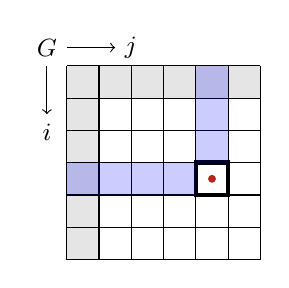
\begin{tikzpicture}[x=4.1mm,y=4.1mm,baseline=(center), remember picture]
  \coordinate(center) at (3,3);
  \draw[step=1] (0,0) grid (6,6);
  \draw[ultra thick] (4,2) rectangle +(1,1);
  %\node(Gij) at (4.5,2.5) {\tiny $\scriptscriptstyle\langle i,j\rangle$};
  \node[circle,fill=BrickRed,inner sep=0,minimum size=1mm](Gij) at (4.5,2.5) {};
  \fill[black,opacity=0.1] (0,5) rectangle (6,6);
  \fill[black,opacity=0.1] (0,0) rectangle (1,5);
  \fill[blue,opacity=0.2] (0,2) rectangle (4,3);
  \fill[blue,opacity=0.2] (4,3) rectangle (5,6);
  \node[anchor=south east](G) at (0,6) {\small$G$};
  \draw[->] (G.east) -- +(1.5,0) node[anchor=west] {\small $j$};
  \draw[->] (G.south) -- +(0,-1.5) node[anchor=north] {\small $i$};
\end{tikzpicture}
&
\small
$
\begin{array}{l@{}}
	\tikz[overlay, remember picture]{\draw[BrickRed] (0,0) -- (Gij);}
	G_{ij} ~=~ \\
	~
	\begin{cases}
		0                        & i=j=0 \\
		\yw{0j0}                  & i=0, j>0 \\
		\xw{0i0}                 & i>0, j=0 \\
		\begin{array}{@{}l@{\hspace{-1pt}}l@{\hspace{-4pt}}}
		  \min\langle & \underset{0\leq q<j}\min ~ G_{iq} + \yw{qji},  \\
		              & \underset{0\leq p<i}\min ~ G_{pj} + \xw{pij}~\rangle
		\end{array}              & i,j>0
	\end{cases}
\end{array}
$
\end{tabular}
\vspace{5pt}
\caption{Recurrence equation and cell-level dependencies.}
\label{intro:arbiter spec}
\end{figure}


The optimal cost for scheduling the first $i$ slots of $x$ and the first $j$ slots
of $y$ is given by the recurrence in \Cref{intro:arbiter spec}. When $i$ is zero, it means that
only $y$ has been scheduled, so the cost is $\yw{0j0}$, and similarly when $j$ is zero, 
the cost is $\xw{0i0}$. When $i$ and $j$ are both positive, there are two options:
either the schedule ends with an allocation to $x$, 
where slots $[p..i)$ of $x$ were scheduled at $t=p+j$, and the cost is 
$G_{pj} + \xw{pij}$; or it ends with an allocation to $y$, where
slots $[q..j)$ of $y$ were scheduled at $t=i+q$, and the cost is $G_{iq} + \yw{qji}$.
The minimum over all respective $p<i$ and $q<j$ is taken.
Eventually, the optimal cost of the entire schedule is given by $G_{|x||y|}$.

\begin{paragraph}{Iterative Algorithm.}
Using a standard dynamic programming method, Richard, an algorithms expert, computes this recurrence
with an iterative program by understanding the dependency pattern:
to compute the $\min\langle\rangle$ expression in \Cref{intro:arbiter spec} and find the optimal
values for $p$ and $q$, the algorithm needs information from all cells above and to the left of $G_{ij}$.
In particular, each value $G_{ij}$ is computed from other values $G_{i'j'}$ with lower
indexes, $i'<i$, ~$j'<j$. 
Therefore, considering $G$ as a two-dimensional array, it can be filled in a single pass from left to right and from top
to bottom.
\end{paragraph}

\newcommand\FORLINE[1]{\STATE\algorithmicfor~{#1} \algorithmicdo~}

\begin{algorithm}
\renewcommand\arraystretch{1.3}
\begin{algorithmic}
  \STATE $G_{00} := 0$
  \FORLINE{$j=1..|y|$}  $G_{0j} := \yw{0j0}$  
  \FOR{$i=1..|x|$}
    \STATE $G_{i0} := \xw{0i0}$
    \FOR{$j=1..|y|$}
      \STATE $G_{ij} :=
        \begin{array}[t]{@{}l@{~}l} 
          \min\langle & \underset{0\leq q<j}\min ~ G_{iq} + \yw{qji}, \underset{0\leq p<i}\min ~ G_{pj} + \xw{pij}~\rangle \\         
        \end{array}$
    \ENDFOR
  \ENDFOR
\end{algorithmic}
\caption{\label{intro:iterative}
   Iterative Simplified Arbiter}
\end{algorithm}


\newcommand\qbox[1]{\fbox{\scriptsize#1}}

\begin{paragraph}{Divide-and-Conquer Algorithm.}

\begin{figure}
\centering
\begin{tabular}{c@{\hspace{.5in}}c}
$
\renewcommand\arraystretch{2}
\begin{array}[b]{c|c|c|c|}
  \multicolumn{2}{c}{} & \multicolumn{2}{c}{J} \\ \cline{3-4}
  \multicolumn{2}{c}{} & \multicolumn{1}{c}{J_0}  & \multicolumn{1}{c}{J_1}\\ \cline{3-4}
  \multirow{2}{*}{$I$} & I_0 & 1 & 2 \\ \cline{3-4}
    & I_1 & 3 & 4 \\ \cline{3-4}
\end{array}
$
& 
$\begin{array}[b]{l}\qbox1 \rightsquigarrow \qbox2 \\ 
\qbox1 \rightsquigarrow \qbox3 \\ \qbox2\rightsquigarrow \qbox4 \\ \qbox3 \rightsquigarrow \qbox4\end{array}$
\end{tabular}
\vspace{5pt}
\caption{\label{intro:quadrants}
  Dividing a two-dimensional array into quadrants; the dependencies are shown on the right.}
\end{figure}

Divide-and-conquer is an algorithm development pattern (\cite{SODA06/Chowdhury}, \cite{SPAA08/Chowdhury})\coa{should these (SODA/SPAA) be the ones to cite here?}, 
where the DP table is partitioned into regions, and each region is expressed as a sub-problem
to be solved.

In our case, Richard takes the two-dimensional array $G$ and partitions it into
quadrants, as illustrated in \Cref{intro:quadrants}. He then applies the same reasoning
as in the iterative case, concluding that the computations of 2 and 3 depend on 1,
and the computation of 4 depends on 2 and 3.
\end{paragraph}

Richard \emph{stratified} the computations on these quadrants into the following
four steps:
\begin{algorithmic}[1]
  \STATE Compute \qbox1 (using only input data $w,w'$).
  \STATE Compute \qbox2 using data from \qbox1.
  \STATE Compute \qbox3 using data from \qbox1.
  \STATE Compute \qbox4 using data from \qbox2 and \qbox3.
\end{algorithmic}

Each step depends only on a subset of the steps that came before it, 
as illustrated by \Cref{intro:chain}. However, this is not yet a divide-and-conquer algorithm: 
of the four steps, only step \qbox1{} is an instance of the original problem; all the other steps
look somewhat different from the original problem and lack significant locality. With some algebraic manipulation, however, 
it is possible to define each of the four steps above recursively, leading to a true divide-and-conquer algorithm with very high locality 
and significantly improved performance relative to the iterative algorithm.

To illustrate how this is done, we first introduce a small amount of notation. 
We define $I$ and $J$ to be the index sets for the rows and columns, respectively.
We then define partitions $I=I_0\cup I_1$ and $J=J_0\cup J_1$ as in \Cref{intro:quadrants}.
$G$ is now parameterized on those index sets;

\begin{equation}
\begin{array}{l@{}l}
	G^{^{IJ}}_{(i:I)\,(j:J)} ~=~  \\
	\qquad
	\begin{cases}
		0                         & i=j=0 \\
		w_{0j0}                   & i=0, j>0 \\
		w'_{0i0}                  & i>0, j=0 \\
		\begin{array}{@{}l@{~}l}
		  \min\langle & \underset{q\in J\cap[0,j)}\min ~ G^{^{IJ}}_{iq} + \yw{qji}, \\
		              & \underset{p\in I\cap[0,i)}\min ~ G^{^{IJ}}_{pj} + \xw{pij}~\rangle
		\end{array}              & i,j>0
	\end{cases}
\end{array}
\end{equation}

The computation of \qbox1 corresponds to computing $G^{IJ}$ within the sub-domain 
$I_0\times J_0$, making it an exact copy of $G^{I_0J_0}$. This is due to the fact
that for $j\in J_0$, ~$J\cap[0,j)=J_0\cap[0,j)$, and for $i\in I_0$, ~$I\cap[0,i)=I_0\cap[0,i)$.

On the other hand, the computation of \qbox2 is {\bf not} a mere copy of $G^{I_0J_1}$, 
because the range $q\in J\cap[0,j)$ is not a subset of $J_1$, so that
some of the recursive references $G_{iq}$ are outside of \qbox2.

This can be addressed by splitting that range, adding yet range another parameter to $G$.

\begin{equation}\LeftEqNo
\begin{array}{l@{}l}
	G^{^{IJJ'}}_{(i:I)\,(j:J)} ~=~  \\
	\qquad
	\begin{cases}
		0                         & i=j=0 \\
		w_{0j0}                   & i=0, j>0 \\
		w'_{0i0}                  & i>0, j=0 \\
		\begin{array}{@{}l@{~}l}
		  \min\langle & \underset{~q\in J'~}\min ~ G^{^{IJ'\!J'}}_{iq} + \yw{qji}, \\
		              & \underset{q\in J'\cap[0,j)}\min ~ G^{^{IJJ}}_{iq} + \yw{qji}, \\
		              & \underset{p\in I\cap[0,i)}\min ~ G^{^{IJJ'}}_{pj} + \xw{pij}~\rangle
		\end{array}              & i,j>0
	\end{cases}
\end{array}
\end{equation}

The computation of \qbox2 is now a copy of $G^{I_0J_1J_0}$. ~$G$ can be further generalized in the following
way:

\newcommand{\Ggen}{H}

\begin{equation}\LeftEqNo
\begin{array}{l@{}l}
	\Ggen^{^{IJ}}_{(i:I)\,(j:J)\,\psi} ~=~  \\
	\qquad
	\begin{cases}
		0                         & i=j=0 \\
		w_{0j0}                   & i=0, j>0 \\
		w'_{0i0}                  & i>0, j=0 \\
		\begin{array}{@{}l@{~}l}
		  \min\langle & \psi_{ij}, \\
		              & \!\underset{q\in J\cap[0,j)}\min ~ G^{^{IJJ}}_{iq} + \yw{qji}, \\
		              & \!\underset{p\in I\cap[0,i)}\min ~ G^{^{IJJ}}_{pj} + \xw{pij}~\rangle
		\end{array}              & i,j>0
	\end{cases}
\end{array}
\label{intro:Ggen}
\end{equation}

It is easy to see that both $G$ and \qbox1 can be expressed in terms of $\Ggen^{IJ}$ by making $\psi_{ij}=\infty$, 
but more importantly, \qbox2 can now also be expressed in terms of $\Ggen^{I_0J_1}$ by making 
$\psi_{ij} =  \underset{q\in J_0}\min ~ G^{I_0J_0J_0}_{iq} + \yw{qji}$.
Moreover, the calls to $G$ inside $\Ggen$ can be replaced with recursive calls to $\Ggen$ itself,
giving the form: 

\begin{equation}\LeftEqNo
\begin{array}{l@{}l}
	\Ggen^{^{IJ}}_{(i:I)\,(j:J)\,\psi} ~=~  \\
	\qquad
	\begin{cases}
		0                         & i=j=0 \\
		w_{0j0}                   & i=0, j>0 \\
		w'_{0i0}                  & i>0, j=0 \\
		\begin{array}{@{}l@{~}l}
		  \min\langle & \psi_{ij}, \\
		              & \!\underset{q\in J\cap[0,j)}\min ~ H^{^{IJ}}_{iq} + \yw{qji}, \\
		              & \!\underset{p\in I\cap[0,i)}\min ~ H^{^{IJ}}_{pj} + \xw{pij}~\rangle
		\end{array}              & i,j>0
	\end{cases}
\end{array}
\end{equation}

The same approach can be used to develop the computations of \qbox3 and \qbox4.
The sub-computation of $\psi$ can also be transformed into four recursive sub-computations, further improving the locality of the resulting algorithm.
So through these kind of transformations, it is possible to break the computation of the original $G$ into four (or more) subcomputations, each of which can be itself recursively partitioned into four subcomputations, giving us a true divide-and-conquer algorithm.
When the pieces become small enough, the iterative algorithm (\Cref{intro:iterative}) is executed.

\medskip
As was outlined in \Cref{divide}, prior work has shown that the performance results that can be achieved through these transformations can be dramatic. Unfortunately, the line of reasoning that was followed in this section can get quite complicated for most dynamic programming algorithms, and producing a correct divide-and-conquer algorithm for a given dynamic programming problem is considered quite difficult even by the researchers who originally pioneered this technique. 

In the following sections, we describe the parts that make Bellmania --- a formal framework for deriving algorithms from specifications. 
It utilizes \newterm{solver-aided tactics} to generate provably correct pseudo-code; 
this approach is demonstrated by engineering specialized tactics for the domain of divide-and-conquer DP.


\begin{figure}
\centering
\begin{tikzpicture}[>=latex,x=6mm,y=6mm,
    every path/.style={step=1},
    every node/.style={inner sep=.5pt},
    block/.style={rectangle,draw,thick,fill=Orange, fill opacity=0.15, inner sep=0}]
    
  \def\dx{1.75cm}
  \def\w{3mm}
    
  \draw (0,0) grid (2,2);
  %\node(1) at (.5,1.5) {1};   \node(2) at (1.5,1.5) {2};
  %\node(3) at (.5,.5) {3};    \node(4) at (1.5,.5) {4};

  \node[inner sep=0] at (2.5,1) {\includegraphics[width=\w]{img/arrow}};

  \tikzset{xshift=\dx}
  
  \draw (0,0) grid (2,2);
  \node(1) at (.5,1.5) {1};   %\node(2) at (1.5,1.5) {2};
  %\node(3) at (.5,.5) {3};         \node(4) at (1.5,.5) {4};
  \node(s)[block,fit={(0,1) (1,2)}] {};
  \node[inner sep=0] at (2.5,1) {\includegraphics[width=\w]{img/arrow}};

  \tikzset{xshift=\dx}
  
  \draw (0,0) grid (2,2);
  \node(1) at (.5,1.5) {1};  \node(2) at (1.5,1.5) {2};
  %\node(3) at (.5,.5) {3};        \node(4) at (1.5,.5) {4};
  \draw (s.70) edge[->,out=20] (2);
  \node(s)[block,fit={(0,1) (1,2)}] {};
  \node[inner sep=0] at (2.5,1) {\includegraphics[width=\w]{img/arrow}};

  \tikzset{xshift=\dx}
  
  \draw (0,0) grid (2,2);
  \node(1) at (.5,1.5) {1};   \node(2) at (1.5,1.5) {2};
  \node(3) at (.5,.5) {3};%    \node(4) at (1.5,.5) {4};
  \draw (s.south) edge[->,out=-40,in=-150] (3.250);
  %\fill[block] (0,0) |- (.9,1) to[out=0,in=-90] (1,1.1) |- (2,2) |- (1.1,1) to[out=180,in=90] (1,.9) |- cycle;
  \coordinate (s) at (.8,0);
  \node[inner sep=0 ] at (2.5,1) {\includegraphics[width=\w]{img/arrow}};

  \tikzset{xshift=\dx};

  \draw (0,0) grid (2,2);
  \node(1) at (.5,1.5) {1};   \node(2) at (1.5,1.5) {2};
  \node(3) at (.5,.5) {3};    \node(4) at (1.5,.5) {4};
  \draw (s.south) edge[->,out=-30,in=-150] (4);
 
\end{tikzpicture}
%\includegraphics[width=.47\textwidth]{img/gap-stratify1}
\caption[caption]{\label{intro:chain}
  Stratified computation for Simplified Arbiter. \\[.2em]
  The array is initially empty; 
  shaded areas indicate the region that is read at each step. }
\end{figure}



\section{Overview}
\label{overview}

Most readers are likely familiar with the Dynamic Programming (DP) technique of Richard Bellman~\cite{03/Bellman:DP} to construct an optimal solution to a problem by combining together optimal solutions to many overlapping sub-problems. The key to DP is to exploit the overlap and reuse computed values to explore exponential-sized solution spaces in polynomial time. Dynamic programs are usually described through recurrence relations that specify how to decompose sub-problems, and is typically implemented using a DP table where each cell holds the computed solution for one of these sub-problems. The table can be filled by visiting each cell once in some predetermined order, but recent research has shown that it is possible to achieve order-of-magnitude performance improvements over this standard implementation approach by developing \emph{divide-and-conquer}  implementation strategies that recursively
partition the space of subproblems into smaller subspaces~\cite{IPDPS15/Tithi,SODA14/Bender,SODA06/Chowdhury,SPAA08/Chowdhury,TOCS10/Chowdhury,TCBB10/Chowdhury}. 

Before delving into how Bellmania supports the process of generating such an implementation, it is useful to understand how a traditional iterative implementation works. For this, we will use the 
optimal parenthesization algorithm from the introduction (\Cref{intro:naive}). The problem description is as follows: given a sequence of factors $a_0\!\cdots a_{n-1}$, 
the goal is to discover a minimal-cost placement of parentheses in the product expression
assuming that multiplication is associative but not commutative. The cost
of reading $a_i$ is given by $x_i$, and that the cost for multiplying
$\Pi(a_{i..(k-1)})$ by $\Pi(a_{k..(j-1)})$ is given by $w_{ikj}$. The specification of the algorithm is shown in \Cref{overview:paren spec}; 
the values $x_i$ and  $w_{ikj}$ are inputs to the algorithm, and the output is a table $G$, where each element $G_{ij}$ is the lowest cost for parenthesizing $a_{i..(j-1)}$, with $G_{0n}$ being the overall optimum.

\begin{figure}[b]
\begin{tabular}{@{\hspace{-4pt}}r@{~~~}p{5cm}@{\hspace{-4pt}}}
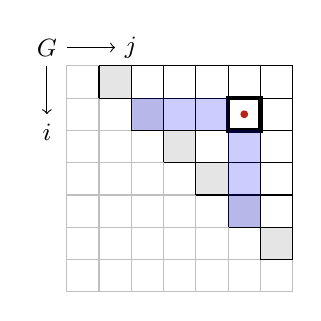
\begin{tikzpicture}[x=4.1mm,y=4.1mm,baseline=(center), remember picture]
  \coordinate(center) at (3,3);
  \def\n{7}  % actually n+1 but let's not be nitpicky
  \draw[black!25!white] (\n,1) |- (0,0) |- (1,\n);
  \draw (\n,1) -- (\n,\n) -- (1,\n);
  \foreach \i [evaluate=\i] in {2-1,...-1,\n-1} {
    \draw[black!25!white] (0,\i) -- (\n-\i,\i); 
    \draw[black!25!white] (\i,0) -- (\i,\n-\i); 
    \draw (\n,\i) -- (\n-\i,\i); 
    \draw (\i,\n) -- (\i,\n-\i);
  }
  %\draw[step=1] (0,0) grid (6,6);
  \draw[ultra thick] (5,5) rectangle +(1,1);
  \node[circle,fill=BrickRed,inner sep=0,minimum size=1mm](Gij) at (5.5,5.5) {};
  \fill[black,opacity=0.1] (1,\n) rectangle ++(1,-1) rectangle ++(1,-1) rectangle ++(1,-1) rectangle ++(1,-1) rectangle ++(1,-1) rectangle ++(1,-1);
  \fill[blue,opacity=0.2] (2,5) rectangle (5,6);
  \fill[blue,opacity=0.2] (5,2) rectangle (6,5);
  \node[anchor=south east](G) at (0,\n) {\small$G$};
  \draw[->] (G.east) -- +(1.5,0) node[anchor=west] {\small $j$};
  \draw[->] (G.south) -- +(0,-1.5) node[anchor=north] {\small $i$};
\end{tikzpicture}
&
\vspace{-1.5cm}
\small
$
\begin{array}{@{}l@{}}
	\tikz[overlay, remember picture]{\draw[BrickRed] (-.5mm,0) -- (Gij);}
	G_{ij} ~=~ \\
	~
	\begin{cases}
		~~x_i                        & i{+}1=j \\
	    \underset{i<k<j}\min ~ G_{ik} {+} G_{kj} {+} w_{ikj} & i{+}1<j
	\end{cases}
\end{array}
$

\vspace{6mm}
% legend
\cbstart
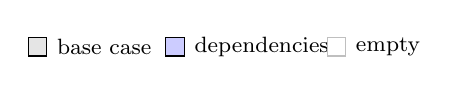
\begin{tikzpicture}
  \node(base)[draw,fill=black!10!white,label=right:{\fontsize{8}{8}\selectfont base case}] {};
  \node(dep)[right=1.5cm of base,draw,fill=blue!20!white,label=right:{\fontsize{8}{8}\selectfont dependencies}] {};
  \node(emp)[right=1.8cm of dep,draw=black!25!white,label=right:{\fontsize{8}{8}\selectfont empty}] {};
\end{tikzpicture}
\cbend
\end{tabular}
\caption{Recurrence equation and cell-level dependencies.}
\label{overview:paren spec}
\end{figure}

\begin{paragraph}{Iterative Algorithm.}
Using the standard dynamic programming method, anyone who has  read \cite{09/CLRS} would compute this recurrence
with an iterative program by understanding the dependency pattern:
to compute the $\min_{i<k<j}(\cdots)$ expression in \Cref{overview:paren spec}
the algorithm needs to enumerate $k$ and gather information from all cells below and to the left of $G_{ij}$.
In particular, each value $G_{ij}$ is computed from other values $G_{i'j'}$ with higher
row indexes $i'>i$ and lower column indexes $j'<j$. 
Therefore, considering $G$ as a two-dimensional array, it can be filled in a single sweep from left to right and from bottom
to top, as done in \Cref{intro:naive}.
\end{paragraph}




\newcommand\qbox[1]{\fbox{\rm\scriptsize#1}}
\newcommand\tinyqbox[1]{\hspace{.5pt}\tikz \node[draw,inner sep=1.5pt] {$\scriptscriptstyle #1$};}

\newcommand\plusoneocd{\raisebox{.5pt}{$\scriptstyle+1$}}

\algrenewtext{Procedure}{\hspace{-3mm}{\bf procedure}~}  % hack to make proc header slighly less indented

\begin{paragraph}{Divide-and-Conquer Algorithm.}
To illustrate the main concepts underlying Bellmania and the key ideas in deriving divide-and-conquer implementations, 
we will walk through the first
few steps that an algorithms expert --- whom we will call Richard --- would follow using Bellmania to generate a provably correct divide-and-conquer implementation of the optimal parenthesization algorithm.

In the Bellmania development model, Richard will start with the specification from \Cref{overview:paren spec}, and progressively manipulate it to get the specification in a form that reflects the recursive structure of the divide-and-conquer implementation. At any step in the transformation, Bellmania can generate code from the partially transformed specification. Code generated from the initial specification will yield an implementation like \Cref{intro:naive}, whereas generating code from the fully transformed specification will yield the divide-and-conquer implementation that we want.
In the rest of the text, we will use the term \newterm{program} to refer to any of the partially transformed specifications.




\begin{figure}
\centering
\begin{tabular}{c@{\hspace{.5in}}c}
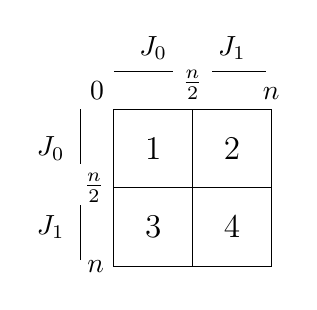
\begin{tikzpicture}[baseline=(n/2), q/.style={font=\relsize{1.3}}, pale/.style={color=black!25!white}]
  % this code draws a grid with the bottom-left paler
  %\draw (0,2) -- (2,2) -- (2,0);
  %\foreach \i in {0,1} {
  %  \draw[pale] (\i,0) -- (\i, 1-\i); \draw (\i,2) -- (\i, 1-\i);
  %  \draw[pale] (0,\i) -- (1-\i, \i); \draw (2,\i) -- (1-\i, \i);
  %}
  % but this might be confusing. let's just paint
  % a regular 2x2 grid
  \draw (0,0) grid (2,2);
  \node[q] at (.5,1.5) {1};   \node[q] at (1.5,1.5) {2};
  \node[q] at (.5, .5) {3};   \node[q] at (1.5, .5) {4};
  \node(O)[above left] at (0,2) {$0$};
  \node(m/2)[above] at (1,2) {$\frac{n}{2}$};
  \node(m)[above] at (2,2) {$n$};
  \node(n/2)[left] at (0,1) {$\frac{n}{2}$};
  \node(n)[left] at (0,0) {$n$};
  \node(J0)[above] at (.5,2.5) {$J_0$};
  \node(J1)[above] at (1.5,2.5) {$J_1$};
  \node(I0)[left] at (-.5,1.5) {$J_0$};
  \node(I1)[left] at (-.5,.5) {$J_1$};
  %\coordinate(0) at (0,0);
  %\coordinate(sw) at (0,0);
  %\coordinate(ne) at (2,2);
  %\draw (J0.north -| sw) -- node[above] {$J$} ++(ne |- 0);
  %\draw (I0.west |- sw) -- node[left] {$I$} ++(ne -| 0);
  \draw (O.north east) -- (O.north east -| m/2.north west);
  \draw (O.north east -| m.110) -- (O.north east -| m/2.north east);
  \draw (O.south west) -- (O.south west |- n/2.north west);
  \draw (O.south west |- n.160) -- (O.south west |- n/2.220);
\end{tikzpicture}
& 
$\begin{array}{l}
  \qbox2 \mbox{\textit{ depends on }} \qbox1 \\[2pt]
  \qbox2 \mbox{\textit{ depends on }} \qbox4 \\ 
  \\
  (\,\qbox3\mbox{\textit{ is empty}})
\end{array}$
\end{tabular}
\vspace{5pt}
\caption{\label{overview:quadrants}
  Dividing a two-dimensional array into quadrants; the dependencies for the case of the running example are shown on the right.}
\end{figure}


\Cref{overview:slice-stratify-synth} provides a visual description of the initial stages of the transformation process. The figure includes block diagrams illustrating how the program at a given stage in the transformation will compute its output table from its input. For example, the first row corresponds to the program before any transformations take place, i.e.~the initial specification. At this stage, the program involves a single loop nest that reads from the entire array and writes to the entire array; solid arrows in the diagram denote data dependency. The transformation from one stage to the next, the dashed arrows, is performed by the application of  \newterm{tactics} that represent a high-level refinement concept. 

As a first step in the transformation, Richard would like to partition the two-di\-men\-sio\-nal array $G$ into quadrants, as illustrated in \Cref{overview:quadrants}. In Bellmania, the partition is accomplished by applying the {\sf Slice} tactic, illustrated graphically at the top of \Cref{overview:slice-stratify-synth}. In order to escape the need to reason about concrete array indices, Bellmania provides an abstract view where
the partitions are labeled $J_0,J_1$. The effect of {\sf Slice} is shown in text in \Cref{overview:logical-slice-stratify}$(a)$ --- the figure trades accuracy for succinctness by omitting the base case of the recurrence for now. Due to the structure of the problem, namely $i\!<\!j$, 
the bottom-left quadrant (\qbox3 in \Cref{overview:quadrants}) is empty.
Slicing therefore produces only three partitions.


The computation of \qbox1
(the top-left quadrant)
does not depend on any of the other computations, so Richard applies the
{\sf Stratify} tactic, which separates an independent computation step as a separate loop. This is equivalent to rewriting the specification as in \Cref{overview:logical-slice-stratify}({\it b}):
the first computation is given a special name $G^{\tinyqbox1}$, then the following
computations read data either from $G^{\tinyqbox1}$ (when the indices are in \qbox1)
or from $G$ (otherwise), which is denoted by $G^{\tinyqbox1}\!/G$. The ``$/\,$'' operator
is part of the Bellmania language and will be defined formally in \Cref{lang}.
Bellmania checks the data dependencies and verifies that the transformation
is sound.

Repeating {\sf Stratify} results in a three-step computation,
as seen in \Cref{overview:slice-stratify-synth}$(c)$, from which Richard can obtain the program in \Cref{overview:breakdown}.
This already gives some performance gain, since computations of \qbox1 and \qbox4 can now run in parallel.
Bellmania is capable of sound reasoning about parallelism, using knowledge encoded
via types of sub-terms, showing that two threads are race-free when they work on different regions
of the table.
This is handled automatically by the code generator.
\end{paragraph}


\begin{figure}
\vspace{-.5em}
\[\renewcommand\arraystretch{1.3}
  \begin{array}{@{}l@{}}
    \textsf{Slice} \quad i,j:\langle J_0\times J_0 \,|\, J_0\times J_1 \,|\, J_1\times J_1\rangle     \hfill (a)\\
    ~~\forall i,j\in\qbox1.~ G_{ij} = \underset{i<k<j}\min ~ G_{ik} + G_{kj} + w_{ikj} \\
    ~~\forall i,j\in\qbox2.~ G_{ij} = \underset{i<k<j}\min ~ G_{ik} + G_{kj} + w_{ikj} \\
    ~~\forall i,j\in\qbox4.~ G_{ij} = \underset{i<k<j}\min ~ G_{ik} + G_{kj} + w_{ikj} \\
    %
    \textsf{Stratify} ~ \qbox1 \hfill (b)\\
    %
    ~~\forall i,j\in\qbox1.~ G^{\tinyqbox1}_{ij} = \underset{i<k<j}\min ~ G^{\tinyqbox1}_{ik} + G^{\tinyqbox1}_{kj} + w_{ikj} \\
    ~~\forall i,j\in\qbox2.~ G_{ij} = \underset{i<k<j}\min ~ (G^{\tinyqbox1}\!/G)_{ik} + (G^{\tinyqbox1}\!/G)_{kj} + w_{ikj} ~~ \\
    ~~\forall i,j\in\qbox4.~ G_{ij} = \underset{i<k<j}\min ~ (G^{\tinyqbox1}\!/G)_{ik} + (G^{\tinyqbox1}\!/G)_{kj} + w_{ikj} \\
  \end{array}
\]
\vspace{-.75em}
\caption{\label{overview:logical-slice-stratify}
  The first two steps in the development, represented as logical specifications.}
\end{figure}


\newcommand\steparrowwidth{3mm}
\newcommand\steparrow{\includegraphics[width=\steparrowwidth]{img/arrow}}

\begin{algorithm}[b]
\renewcommand\arraystretch{1.3}
\begin{algorithmic}
\Procedure{A{\larger{[}}$G${\larger{]}}}{}\EndProcedure
  \For{$i=(n{-}2)..0 \cap J_0$}    \Head{Compute \qbox1}
    \For{$j=(i{+}2)..n \cap J_0$} 
      \State $G_{ij} :=
          \underset{i<k<j}\min ~ G_{ik} + G_{kj} + w_{ikj}$
    \EndFor
  \EndFor
  \For{$i=(n-2)..0 \cap J_1$}    \Head{Compute \qbox4}
    \For{$j=(i{+}2)..n \cap J_1$} 
      \State $G_{ij} :=
          \underset{i<k<j}\min ~ G_{ik} + G_{kj} + w_{ikj}$
    \EndFor
  \EndFor
  \For{$i=(n{-}2)..0 \cap J_0$}    \Head{Compute \qbox2}
    \For{$j=(i{+}2)..n \cap J_1$}
      \State $G_{ij} :=
          \underset{i<k<j}\min ~ G_{ik} + G_{kj} + w_{ikj}$
    \EndFor
  \EndFor
\end{algorithmic}
\caption[t]{\label{overview:breakdown}
   \cbstart Parenthesis\cbend{} --- Sliced and Stratified}
\end{algorithm}


\newbox\primebox
\setbox\primebox\hbox{$'$}
\newbox\doubleprimebox
\setbox\doubleprimebox\hbox{$''$}

\newcommand\primeocd[1]{\hspace{\wd\primebox}#1\usebox\primebox}
\newcommand\doubleprimeocd[1]{\hspace{\wd\doubleprimebox}#1\usebox\doubleprimebox}

\begin{figure}
\centering
\begin{tikzpicture}[>=latex,x=6mm,y=6mm,
    every path/.style={step=1},
    every node/.style={inner sep=.5pt},
    init data/.style={pattern=north west lines, pattern color=green!50!black},
    block/.style={rectangle,draw,very thick,fill=Orange, fill opacity=0.2, inner sep=0},
    knob/.style={midway,draw,fill=white,midway,inner sep=1.25pt}]
    
  \def\dx{1.75cm}
  \def\dy{1.75cm}
  
  % -------------------------------------------------------

  \draw (0,0) rectangle (2,2);
  \node(s)[block,fit={(0,0) (2,2)}] {};
  \node[inner sep=3mm](0) at (1,1) {0};

  \node[inner sep=0] at (2.5,1) {\steparrow};

  \tikzset{xshift=\dx}

  \draw (0,0) rectangle (2,2);
  \node[inner sep=3mm](0) at (1,1) {0$'$};
  \draw (s.70) edge[->,out=20] (0);

  \applytacticnode{Slice ~~ $i : \langle I_0|I_1\rangle$ ~~ $j : \langle J_0|J_1\rangle$};

  \tikzset{yshift=-\dy,xshift=-\dx}
    
  % -------------------------------------------------------

  \draw (0,0) grid (2,2);
  \node(1) at (.5,1.5) {1};   \node(2) at (1.5,1.5) {2};
  \node(3) at (.5, .5) {3};   \node(4) at (1.5, .5) {4};
  \node(s)[block,fit={(0,0) (2,2)}] {};

  \node[inner sep=0] at (2.5,1) {\steparrow};

  \tikzset{xshift=\dx}

  \draw (0,0) grid (2,2);
  \node(1) at (.5,1.5) {\primeocd 1};   \node(2) at (1.5,1.5) {\primeocd 2};
  \node(3) at (.5, .5) {\primeocd 3};   \node(4) at (1.5, .5) {\primeocd 4};
  \draw (s.70) edge[->,out=20] (1);
  \draw (s.70) edge[->,out=20] (2);
  \draw (s.70) edge[->,out=20] (3);
  \draw (s.70) edge[->,out=20] (4);

  \applytacticnode{Stratify \qbox1};

  % -------------------------------------------------------
  \setlength\baselineskip{15pt}  

  \tikzset{yshift=-\dy,xshift=-\dx}

  \draw (0,0) grid (2,2);
  \node(s)[block,fit={(0,1) (1,2)}] {};
  \node(1) at (.5,1.5) {1};   \node(2) at (1.5,1.5) {2};
  \node(3) at (.5, .5) {3};   \node(4) at (1.5, .5) {4};

  \node[inner sep=0] at (2.5,1) {\steparrow};

  \tikzset{xshift=\dx}
  
  \draw (0,0) grid (2,2);
  \node(1) at (.5,1.5) {\primeocd 1};   \node(2) at (1.5,1.5) {2};
  \node(3) at (.5, .5) {3};             \node(4) at (1.5,.5) {4};
  \draw (s.70) edge[->,out=20] node[knob,circle] {} (1);
  \node(s)[block,fit={(0,0) (2,2)}] {};
  
  \node[inner sep=0] at (2.5,1) {\steparrow};

  \tikzset{xshift=\dx}

  \draw (0,0) grid (2,2);
  \node(1) at (.5,1.5) {\primeocd 1};   \node(2) at (1.5,1.5) {\primeocd 2};
  \node(3) at (.5, .5) {\primeocd 3};   \node(4) at (1.5, .5) {\primeocd 4};
  \draw (s.70) edge[->,out=20] (2);
  \draw (s.70) edge[->,out=20] (3);
  \draw (s.70) edge[->,out=20] (4);
  
  \applytacticnode{Synth $\circ ~~ \dashrightarrow A^{I_0J_0}$ \\ 
      \applytactic{Stratify \qbox2}};
  
  \tikzset{yshift=-\dy,xshift=-2*\dx}

  % -------------------------------------------------------

  \draw (0,0) grid (2,2);
  \node(s)[block,fit={(0,1) (1,2)}] {};
  \node(1) at (.5,1.5) {1};   \node(2) at (1.5,1.5) {2};
  \node(3) at (.5, .5) {3};   \node(4) at (1.5, .5) {4};

  \node[inner sep=0] at (2.5,1) {\steparrow};

  \tikzset{xshift=\dx}
  
  \draw (0,0) grid (2,2);
  \node(1) at (.5,1.5) {\primeocd 1};   \node(2) at (1.5,1.5) {2};
  \node(3) at (.5, .5) {3};   \node(4) at (1.5, .5) {4};
  \draw (s.70) edge[->,out=20] node[knob,circle] {} (1);
  \node(s)[block,fit={(0,1) (2,2)}] {};
  \node[inner sep=0] at (2.5,1) {\steparrow};

  \tikzset{xshift=\dx}
  
  \draw (0,0) grid (2,2);
  \node(1) at (.5,1.5) {\primeocd 1};  \node(2) at (1.5,1.5) {\primeocd 2};
  \node(3) at (.5,.5) {3};             \node(4) at (1.5,.5) {4};
  \draw (s.70) edge[->,out=20] (2);
  \node[inner sep=0] at (2.8,1) {$\cdots$};

  \tikzset{xshift=.25*\dx}

  \node[right,align=left] at (3,1) {\applytactic{Slice \qbox2 \\ \quad $p : \langle J_0|J_1\rangle$}};

  \tikzset{yshift=-\dy,xshift=-2.25*\dx}

  % -------------------------------------------------------

  \draw (0,0) grid (2,2);
  \node(s)[block,fit={(0,1) (1,2)}] {};
  \node(1) at (.5,1.5) {1};   \node(2) at (1.5,1.5) {2};
  \node(3) at (.5, .5) {3};   \node(4) at (1.5, .5) {4};

  \node[inner sep=0] at (2.5,1) {\steparrow};

  \tikzset{xshift=\dx}
  
  \draw (0,0) grid (2,2);
  \node(1) at (.5,1.5) {\primeocd 1};   \node(2) at (1.5,1.5) {2};
  \node(3) at (.5, .5) {3};   \node(4) at (1.5, .5) {4};
  \draw (s.70) edge[->,out=20] node[knob,circle] {} (1);
  \node(s1)[block,fit={(0,1) (1,2)}] {};
  \node(s2)[block,fit={(1,1) (2,2)}] {};
  
  \node[inner sep=0] at (2.5,1) {\steparrow};

  \tikzset{xshift=\dx}
  
  \draw (0,0) grid (2,2);
  \node(1) at (.5,1.5) {\primeocd 1};  \node(2) at (1.5,1.5) {\primeocd 2};
  \node(3) at (.5,.5) {3};             \node(4) at (1.5,.5) {4};
  \draw (s1.70) edge[->,out=20] (2);
  \draw (s2.70) edge[->,out=20] (2);
  \node[inner sep=0] at (2.8,1) {$\cdots$};

  \tikzset{xshift=.25*\dx}

  \node[right,align=left] at (3,1) {\applytactic{Stratify \qbox2$^{\# 1}$}};

  \tikzset{yshift=-\dy,xshift=-2.25*\dx}

  % -------------------------------------------------------

  \draw (0,0) grid (2,2);
  \node(s)[block,fit={(0,1) (1,2)}] {};
  \node(1) at (.5,1.5) {1};   \node(2) at (1.5,1.5) {2};
  \node(3) at (.5, .5) {3};   \node(4) at (1.5, .5) {4};

  \node[inner sep=0] at (2.5,1) {\steparrow};

  \tikzset{xshift=\dx}
  
  \draw (0,0) grid (2,2);
  \node(1) at (.5,1.5) {\primeocd 1};   \node(2) at (1.5,1.5) {2};
  \node(3) at (.5, .5) {3};   \node(4) at (1.5, .5) {4};
  \draw (s.70) edge[->,out=20] node[knob,circle] {} (1);
  \node(s)[block,fit={(0,1) (1,2)}] {};
  
  \node[inner sep=0] at (2.5,1) {\steparrow};

  \tikzset{xshift=\dx}
  
  \draw (0,0) grid (2,2);
  \node(1) at (.5,1.5) {\primeocd 1};  \node(2) at (1.5,1.5) {\primeocd 2};
  \node(3) at (.5,.5) {3};             \node(4) at (1.5,.5) {4};
  \draw (s.70) edge[->,out=20] node[knob,isosceles triangle,rotate=90] {} (2);
  \node(s)[block,fit={(1,1) (2,2)}] {};

  \node[inner sep=0] at (2.5,1) {\steparrow};

  \tikzset{xshift=\dx}
  
  \draw (0,0) grid (2,2);
  \node(1) at (.5,1.5) {\primeocd 1};  \node(2) at (1.5,1.5) {\doubleprimeocd 2};
  \node(3) at (.5,.5) {3};             \node(4) at (1.5,.5) {4};
  \draw (s.70) edge[->,out=20] node[knob,diamond] {} (2);
  \node[inner sep=0] at (2.8,1) {$\cdots$};

  \tikzset{xshift=-1.25*\dx,yshift=-.75*\dy}

  \applytacticnode{Synth {\tikz\node[knob,isosceles triangle,rotate=90] {};} $~~ \longrightarrow B^{I_0J_0J_1}$ \\ 
      \applytactic{Synth $\diamond$} $~~ \dashrightarrow A^{I_0J_1}$};

  \tikzset{yshift=-\dy,xshift=-2*\dx}

\end{tikzpicture}

\caption[caption]{\label{overview:slice-stratify-synth}
  Overview of tactic semantics in Bellmania.}
\end{figure}


\medskip
At this point, Richard notices that $G^{\tinyqbox1}$ is just a smaller version of
the entire array $G$; he invokes another tactic called {\sf Synth}, which automatically
synthesizes a recursive call A\big[$G^{\tinyqbox1}$\big]
(presented using abstract index ranges as $A^{J_0}$).

Similarly, $G^{\tinyqbox4}$ is also a smaller version of $G$, this time with
indices from $J_1$. {\sf Synth} figures it out automatically as well,
synthesizing a call A\big[$G^{\tinyqbox4}$\big]. The remaining part,
$G^{\tinyqbox2}$, is essentially different, so Richard gives it a new name, ``B'',
which becomes a new synthesis task.%
\footnote{Richard's choice of names is consistent with the literature.}

\begin{algorithm}[b]
\renewcommand\arraystretch{1.3}
\begin{algorithmic}
\Procedure{A{\larger{[}}$G${\larger{]}}}{}\EndProcedure
  \If{$G$ {\it is very small}} {\it run iterative version}
  \Else
  \State A\big[$G^{\tinyqbox1}$\big] \Head{Compute \qbox1}
  \State A\big[$G^{\tinyqbox4}$\big] \Head{Compute \qbox4}
  \State B\big[$G^{\tinyqbox1}, G^{\tinyqbox4}, G^{\tinyqbox2}$\big] \Head{Compute \qbox2}
  \EndIf
\end{algorithmic}
\caption{\label{overview:recursive-A}
   Parenthesis --- Recursive Version}
\end{algorithm}


Applying the same strategy will eventually lead Richard to further
break down and transform the computation of B into multiple recursive
sub-computations, %\rch{B makes eight recursive function calls to update the four quadrants. So it reduces to eight recursive sub-computations, right?}, 
further improving the locality of the resulting algorithm until
a true divide-and-conquer solution is obtained.
Bellmania generates code for
all procedures encountered throughout the development. In this case, three recursive procedures
are generated. The base case of the recursion is when the region
becomes small enough to just run the loop version.\footnote{The optimal  base case size of the region can be found by auto-tuning (taken as an input in the current version of the compiler)}

As is well illustrated by the example, this line of reasoning can get quite complicated for most dynamic programming algorithms, 
and producing a correct divide-and-conquer algorithm for a given dynamic programming problem is considered quite difficult even by the researchers who originally pioneered the technique. 
Fortunately, Bellmania is able to mechanize most of the technical details,
allowing Richard and other algorithm designers to focus on their area of expertise,
try different strategies,
and eventually produce a \emph{certified} implementation of the algorithm.

Overall, it took Richard only 4 steps to construct \Cref{overview:recursive-A},
and a total of 30 steps to construct all three phases of the Parenthesis algorithm,
comprising an implementation that is 46$\times$ faster than a parallel implementation of
\Cref{intro:naive} using a state-of-the-art parallelizing compiler.
The user is greatly assisted by tactics like {\sf Synth}, which carries out the monotonic
and error-prone task of choosing the right parameters for each recursive call; also,
mistakes are identified early in the development thanks to automatic verification,
saving hours of debugging later on.
The resulting code is much easier to maintain, because the artifact is not just
the optimized C++ code, but also the Bellmania specification and the script
that encodes the optimization strategy.

Once a divide-and-conquer algorithm is found, generating an optimal implementation still requires some additional work, such as finding the right point at which to switch to an iterative algorithm to leverage SIMD parallelism as well as low-level tuning and compiler optimization;
these steps are performed by more traditional compiler optimization techniques
as discussed in \Cref{codegen}.


\subsection*{System Design}

\begin{figure}
  \centering
  
  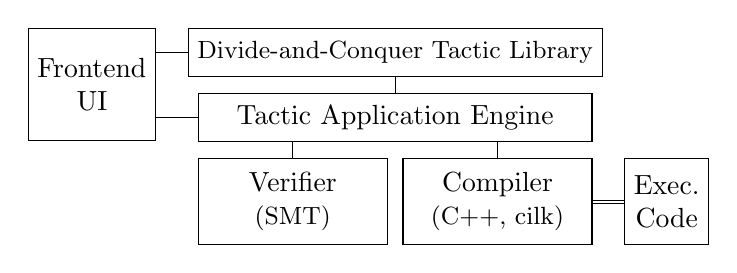
\begin{tikzpicture}[
      h/.style={minimum height=1.75em}, 
      tallh/.style={minimum height=3.1em}, 
      doubleh/.style={minimum height=3.5em+2mm}, 
      fullw/.style={minimum width=5cm}, 
      halfw/.style={minimum width=2.4cm},
      75w/.style={minimum width=1.15cm},
      every node/.style={align=center}]
    \node[draw, h, fullw](tae) {Tactic Application Engine};
    \node[draw, h, fullw, above=2mm of tae](dp) {\fontsize{9.5}{11}\selectfont Divide-and-Conquer Tactic Library};
    \node[draw, tallh, halfw, below=2mm of tae.south west, anchor=north west](verif) {Verifier \\ {\small (SMT)}};
    \node[draw, tallh, halfw, below=2mm of tae.south east, anchor=north east](comp) {Compiler \\ {\small (C++, cilk)}};
    \draw (dp.south) -- (tae.north);
    \draw (tae.south -| verif.north) -- (verif.north);
    \draw (tae.south -| comp.north) -- (comp.north);
    
    \node[draw, doubleh, left=4mm of dp.north west, anchor=north east](ui) {Frontend \\ UI};
    \draw (dp.west) -- (dp.west -| ui.east);
    \draw (tae.west) -- (tae.west -| ui.east);
    
    \node[draw, tallh, right=4mm of comp](exe) {Exec. \\ Code};
    \draw[double] (comp) -- (exe);
  \end{tikzpicture}
\caption{\label{overview:design}
  Overall design of Bellmania.}
\end{figure}

The design of the Bellmania system (\Cref{overview:design}) contains a generic
core --- called the \newterm{Tactic Application Engine} (TAE) ---
on top of which a library of \newterm{tactics} specific to dynamic programming
is built. While it is possible to extend the library, it already contains enough tactics to successfully develop algorithms for a
family of problems, so that the user of the system only needs to apply existing tactics by issuing commands
through a GUI and watching the program evolve. The TAE has a back-end that
verifies conjectures, and is in charge of making sure that
tactic applications represent valid rewritings of the program. Finally, the
programs created this way are transferred to a compilation back-end, where
some automatic static analysis is applied and then executable (C++) code is emitted.

\cbstart\diffnote{made the point clear regarding verification vs. certification, and what is missing}%
The trusted core is small, comprising of:
\begin{enumerate*}[label=(\textit{\alph*})]
 \item a type checker (see \Cref{lang:types}), 
 \item a term substitution procedure (see \Cref{tactics}),
 \item a formula simplifier (see \Cref{automated:simplification}),
 \item the SMT solver, and
 \item the compiler (see \Cref{codegen}).
\end{enumerate*}
In its current version, Bellmania does not emit machine-checkable
proofs; to the extent that SMT solvers can emit such proofs,
these could be adapted to a proof of refinement (in the sense of \cite{POPL15/Delaware}).
The compiler has to be formally verified separately.
These two tasks require considerable engineering effort and are left for the future.
\cbend

\begin{figure}
\vspace{-.5em}% why is there extra space above lstlisting?
\begin{lstlisting}[language=bellmania]
Slice (find (\theta |-> ?)) (? <|J_0*J_0, J_0*J_1, J_1*J_1|>)
Stratify "/" (fixee [A]) [A] \psi
Stratify "/" (fixee [A]) [A] \psi
[A] [B] [C] |-> SynthAuto . ... \psi
\end{lstlisting}
\caption{\label{overview:script}
  Bellmania script used to generate \Cref{overview:recursive-A}.}
\end{figure}

An example for the concrete syntax is shown in \Cref{overview:script}.
A full listing of the scripts for our running examples,
as well as screenshots of the UI, can be found
in \Cref{annex:example:paren}.

\subsection*{Interaction Model}

\begin{figure}[b!]
\begin{tikzpicture}[>=latex,
     blk/.style={draw,rectangle,align=center,inner sep=5pt,minimum height=8mm}]
  \node(spec)[blk]{Specification};
  \node(prog)[blk,below right=8mm of spec]{Program Term};
  \node(deriv)[blk,above=of prog]{Derived\\Definition};
  \node(impl)[blk,above right=8mm of prog]{Implementation};
  \draw[->,rounded corners=5mm] (spec) |- node[below]{\textit{typecheck}} (prog);
  \draw[->] (prog) edge[out=112,in=-105] (deriv);
  \draw[->] (deriv) edge[out=-73,in=70] (prog);
  \draw[->,rounded corners=5mm] (prog) -| node[below]{\textit{compile}} (impl);
  % Loop over (prog)
  \draw[->,rounded corners=3mm] (prog.-10) -| ++(.3,-.6) -| ($(prog.190) + (-.3,0)$) -- (prog.190);
  \node[below=6mm of prog]{\textit{apply tactic}};
\end{tikzpicture}
\caption{\label{overview:flow}
  Interaction workflow in Bellmania.}
\end{figure}

\cbstart\diffnote{added subsection (incl. figure)}%
The intended use pattern for Bellmania is by repeatedly issuing
commands to apply tactics inside a REPL that keeps showing to the
user the resulting \newterm{program term} (\Cref{overview:flow}).
To begin the interaction, the user types in a \newterm{specification} written
in the Bellmania language (as defined in \Cref{lang}), which is typechecked
by the system, producing a term.
This term then becomes the focus of the development, and further transformations
apply to it; the user issues \newterm{apply tactic} commands, one at a time,
using a syntax similar to \Cref{overview:script}.
Tactic applications are also typechecked, as well as the resulting program,
since type information can be refined by including the context (see \Cref{lang:types}).
During the development, sub-computations may be discovered that require
further drilling down (such as ``B'' in the last example).
These result in \newterm{derived} terms that take the focus until they, too,
have been fully transformed.
When the program and all its sub-computations are fully developed and
expressed as a divide-and-conquer algorithm, the user invokes the compiler
back-end that emits C++ code.

In the following sections, we describe the programming language and
formally define the tactics that were used in the example above.
We then show how to formalize the same intuition as we had there,
using this new instrument.
\cbend

\section{A Unified Language}
\label{lang}

\newcommand\semp[1]{[\![{#1}]\!]}
\newcommand\fix{\operatorname{fix}}

We first set up a formal language that we will use to describe computations and reason about them.
Bellmania uses the same language for specifications and for programs.  Its core is the polymorphic
$\lambda$-calculus, that is, simply typed $\lambda$-calculus with universally quantified type variables 
(also known as \newterm{System F}).

We write abstraction terms as $(v:\T)\mapsto e$, where $\T$ is the type of the argument $v$ and $e$ is
the body, instead of the traditional notation $\lambda(v:\T).\,e$, mainly due to aesthetic reasons
but also because we hope this will look more familiar to intended users.
Curried functions $(v_1:\T_1)\mapsto (v_2:\T_2) \mapsto \cdots \mapsto (v_n:\T_n) \mapsto e$ are abbreviated 
as $(v_1:\T_1)\cdots(v_n:\T_n)\mapsto e$.

The semantics differ slightly from that of traditional functional languages: arrow types $\T_1\to\T_2$
are interpreted as {\bf mappings} from values of type $\T_1$ to values of type $\T_2$. Algebraically,
interpretations of types, $\semp{\T_1}$, $\semp{\T_2}$, are sets, and interpretations of arrow-typed terms,
$f : \T_1\to\T_2$, are {\bf partial functions} --- $\semp{f} : \semp{\T_1}\rightharpoonup\semp{\T_2}$.
This implies that a term $t : \T$ may have an \newterm{undefined} value, $\semp{t}=\bot_\T$
(We would shorten it to $\semp{t}=\bot$ when the type is either insignificant or understood from the context).
For simplicity, we shall identify $\bot_{\T_1\to\T_2}$ with the empty mapping $(v:\T_1)\mapsto\bot_{\T_2}$.

All functions are naturally extended, so that $f\,\bot=\bot$.

\subsection{Operators}
\label{lang:operators}

The core is augmented with the following intrinsic operators:

\begin{itemize}
  \item A fixed point operator $\fix f$, with the denotational semantics
    \[\semp{\fix f} ~=~ \theta \textrm{ ~ s.t. ~ } \semp f\,\theta=\theta\]
  we assume that recurrences given in specifications are well-defined, 
  such that $\semp f$ has a single fixed point.
  In other words, we ignore nonterminating computations.
  \item A guard operator $[\,]_{_\square}\,$, which comes in two flavors:
  \[\begin{array}{l}
      [x]_{\mathit{cond}} = \begin{cases}x & \mathit{cond} \\ \bot & \lnot\mathit{cond}\end{cases} \\
      {}[f]_{P_1\times P_2\times \cdots P_n} = \overline{x} \mapsto [f\,\overline{x}]_{\bigwedge P_i(x_i)}
    \end{array}\]
  where $\overline{x} = x_1 \cdots x_n$. This second form can be used to
  refer to quadrants of an array; for example, in \Cref{overview:quadrants-abstract}, $\qbox2 \equiv [G]_{J_0\times J_1}$.
  \item A slash operator $/$,     \vspace{-2pt}
  \[\renewcommand\arraystretch{1.5}
    \begin{array}{ll}
      \mbox{For scalars $x,y:\S$} & x/y = \begin{cases}x & \mbox{if }x\neq\bot \\ y & \mbox{if }x=\bot\end{cases} \\
      \mbox{For $f,g:\T_1\to\T_2$} & f/g = (v:\T_1)\mapsto (f\,v)/(g\,v)
    \end{array}\]
  This operator is typically used to combine computations done on
  parts of the array. For example, \[\psi\mapsto \big[f\,\psi\big]_{I_0} ~ \Big/ ~ \big[g\,\psi\big]_{I_1}\]
  combines a result of $f$ in the lower indices of a (one-dimensional) array
  with a result of $g$ in the higher indices ($I_0$ and $I_1$, respectively, are the index subsets).
  Notice that this does not limit the areas from which $f$ and $g$ read,
  and they are free to access the entire domain of $\psi$.
\end{itemize}

In our concrete syntax, function application takes precedence over $/$,
and the bodies of $\mapsto$ spans as far as possible.

\subsection{Primitives}

The standard library contains some common primitives:

\begin{itemize}
  \item $\R$, a type for real numbers; $\N$ for natural numbers; $\B$ for Boolean true/false.
  \item ${=} : \T\to\T\to\B$, always interpreted as equality.
  \item ${+}, {-} : \T\to\T\to\T$, polymorphic binary operators.
  \item ${<} : \T\to\T\to\B$, a polymorphic order relation.
  \item $cons : \T\to(\N\to\T)\to(\N\to\T), nil : \N\to\T$, list constructors.
  \item $\min, \max, \Sigma : (\T\to\S)\to\S$, reduction (aggregation) operators
    on ordered/unordered collections. The collection is represented by a mapping $f : \T\to\S$,
    so that e.g. \[\semp{\min f} = \min \big\{\semp{f}\,v \;\big|\; v\in\semp{\T}, \semp{f}\,v\neq\bot\big\}\]
    The collections are expected to be finite.
\end{itemize}

\subsection{Additional Notation}
\newcommand\applt{\textrm{{\scriptsize\,}\guillemotright{\scriptsize\,}}}

We also adopt some syntactic sugar to make complex terms more managable:

\begin{itemize}
  \item $x \applt f ~=~ f\,x$ for application from the left.
  \item $\langle t_1,\cdots,t_n\rangle = cons~t_1 ~ (cons \cdots (cons~t_n ~ nil) \cdots)$
    for fixed-length lists.
\end{itemize}

\subsection{Types and Type Qualifiers}

We extend the type system with predicate abstraction in the form of logically qualified data types 
(Liquid Types~\cite{PLDI08/Rondon}). These are refinement types restricted via a set of abstraction predicates,
called \newterm{qualifiers}, which are defined over the base types.
Contradictory to the general use of refinement types, the purpose of these qualifiers is not to
check a program for safety and reject ill-typed program, but rather to serve as annotations for
tactics, to convey information to the solver for use in the proof, and later to help the compiler
to properly schedule parallel computations.

More specifically, typing $f : \{v:\T_1 ~|~ P(v)\}\to\T_2$ would mean that $f\,x$
can only be defined where $P(x)$ is true; otherwise, $f\,x=\bot$. 
It {\bf does not} mean that the compiler has to prove $P(x)$ at the point where the term $f\,x$
occurs.

As such, we define a Bellmania program to be well-typed iff it is well-typed
without the annotations (in its \newterm{raw form}). Qualifiers are processed
as a separate pass to properly annotate sub-terms.

Some qualifiers are built-in, and more can defined by the user. To keep the syntax simple, we somewhat
limit the use of qualifiers, allowing only the following forms:

\begin{itemize}
  \item $\{v:\T ~|~ P(v)\}$, abbreviated as $\T\cap P$. When the signature of $P$ is known (which is
  almost always), it is enough to write $P$.
  \item $\{v:\T ~|~ P(v)\land Q(v)\}$, abbreviated as $\T\cap P\cap Q$, or just $P\cap Q$. This extends
  to any number of conjuncts of the same form.
  \item $(x : \T_2) \to \{v:\T_2 ~|~ R(x,v)\} \to \T_3$, abbreviated as $\big((\T_1\times\T_2)\cap R\big)\to\T_3$.
  The qualifier argument $x$ must be the preceding argument; this extends to predicates of
  any arity (that is, a $k$-ary predicate in a qualifier is applied to the $k$
  arguments to the left of it, including the one where it appears).
\end{itemize}


\medskip  
The type refinement operators $\cap$ and $\times$ may be composed to create \newterm{droplets},
using the abstract syntax in \Cref{lang:droplets}.
Note that the language does not define tuple types; hence there is no distinction between curried and uncurried function types.
Droplets can express conjunctions of qualifiers,
as long as their argument sets are either disjoint or contained, but not overlapping;
for example, \[x:\{v:\T_1~|~P(v)\}\to \{v:\T_2~|~Q(v)\land R(x,v)\}\to\T_3\] can be written as
$\big((P\times Q)\cap R\big)\to\T_3$, but \[x:\T_1\to y:\{v:\T_2~|~R(x,v)\} \to \{v:\T_3~|~R(y,v)\}\to\T_4\]
cannot be represented as a droplet.

As with any refinement type system, we define the \newterm{shape} of a droplet to be the raw type
obtained from it by removing all qualifiers.

\newcommand\examplePar{%
\noindent\hspace{-2pt}%
\tikz[baseline=(E.base)]\node(E)[draw,rectangle,rounded corners=.7em] {\bf Example};
}
\examplePar
The inputs $\xw{}$, $\yw{}$ to the Simplified Arbiter (\Cref{intro:arbiter spec}) can be typed using these droplets:
\[
\begin{array}{l}
  \xw{} : ((I\times I)\cap{<})\to J\to\R \\
  \yw{} : ((J\times J)\cap{<})\to I\to\R
\end{array}
\]

This states that $w\,p\,i\,j$ is only defined for $p<i$. It doesn't {\em force} it to be defined,
as it is still a partial function. This property is in fact useful: we now have a mechanism for
specifying that some schedules are impossible, by setting the respective $w\,p\,i\,j=\bot$!

\subsubsection*{Typing Rules}

\begin{figure}
\[
\begin{array}{lcll}
  d       & ::= & e^1 \quad |\quad e^k\to d \\
  e^1     & ::= & \T & \mbox{\it\small for scalar type $\T$} \\
  e^{k+l} & ::= & e^k \times e^l \\
  e^k     & ::= & e^k \cap P & \mbox{\it\small for $k$-ary predicate symbol $P$} 
\end{array}
\]
\vspace{-.5em}
\caption{\label{lang:droplets}
  Syntax of type qualifiers (droplets). $k$, $l$ are positive integers
  that stand for dimension indexes.}
\end{figure}

As mentioned earlier, annotations are ignored when typechecking a term.
This gives a simple characterization of type safety without the need to
explictly write any new typing rules. It also means that for $f:\T_1\to\T_2$, $x:\T_3$, we obtain $f\,x:\T_2$ whenever
$\T_1$ and $\T_3$ have the same shape. This requires some explanation.

Considering a (partial) function $\T\to\S$ to be a set of pairs of elements $\langle x,y\rangle$ 
from its domain $\T$ and range $\S$, respectively, it is clear to see that any function of type $\T_1\to\S_1$,
such that $\semp{\T_1}\subseteq\semp{\T}$, $\semp{\S_1}\subseteq\semp{\S}$, 
is \emph{also}, by definition, a function of type $\T\to\S$, since $\semp{\T_1}\times\semp{\S_1}\subseteq\semp{\T}\times\semp{\S}$.
If we define subtyping as inclusion of the domains, i.e. $\T_1 <:\T$ whenever $\semp{\T_1}\subseteq\semp{\T}$,
this translates into:
%
\[\T_1<:\T ~\land~ \S_1<:\S ~~\Rightarrow~~ (\T_1\to\S_1) <: (\T\to\S)\]

In this case, the type constructor $\to$ is {\bf covariant} in both arguments.\footnote{This is different from classical view, and holds in this case because we interpret functions as \emph{mappings}.}
With this in mind, a function $g:(\T\to\S)\to \S_2$ can be called with an argument $a: \T_1\to\S_1$,
by regular subtyping rules, and $g\,a : \S_2$.

When the argument's type is not a subtype, but has the same shape as that of the expected type,
it is \newterm{coerced} to the required type by restricting the values to the desired proper subset.
%
\[\mbox{For }h:\T\to\S \qquad \semp{h\,a} ~=~ \semp{h}\big(\semp{a} :: \T\big)\]

Where $::$ is defined as follows:
\begin{itemize}
  \item For scalar (non-arrow) type $\T$, \[x :: \T ~=~ \begin{cases}x & \mbox{if }x\in\semp{\T} \\ \bot & \mbox{if }x\not\in\semp{\T}\end{cases}\]
  \item $f :: \T\to\S ~=~ x\mapsto \big(f\,(x :: \T)\big) :: \S$
\end{itemize}

\medskip
We extend our abstract syntax with an explicit \newterm{cast operator}
$t::\T$ following this semantics. Notice that the second case of $[\,]_{_\square}\,$
can be defined as syntactic sugar for $::$,
$[t]_{_\square} = t :: \square\to \_$, where $\_$ is a fresh
type variable to be inferred.

\subsubsection*{Type Inference}

Base types are inferred normally as in a classical Hindley-Milner type system.
The operators (\Cref{lang:operators}) behave like polymorphic
constants with the following types:
\[\renewcommand\arraystretch{1.5}
  \begin{array}{c}
    {\fix} : (\T\to\T)\to\T \qquad {/} : \T\to\T\to\T \\
    (::\T) : \mathrm{shape}[\T]\to\mathrm{shape}[\T]
  \end{array}\]

Any type variables occurring in type expressions are resolved at that
stage. In particular, it means that type variables are always assigned raw types.

Qualifiers are also inferred by essentially propagating them up and down the syntax tree.
Since the program already typechecks once the base types are in place, the problem is no longer
one of finding {\em valid} annotations, but rather of {\em tightening} them as much as possible
without introducing semantics-changing coercions. For example, $(f :: I\to(I\cap P))\,i$ may
be assigned the type $I$, but it can also be assigned $I\cap P$ without changing its semantics.

Qualifiers are propagated by defining a \newterm{type intersection} operator $\sqcap$ that
takes two droplets of the same shape $\T_1$, $\T_2$ and returns a droplet with a conjunction of all the qualifiers
occuring in either $\T_1$ or $\T_2$. The operator is defined in terms of the corresponding liquid types:
\begin{itemize}
  \item If $\T_1=\{v:\T ~|~ \varphi_1\}$ and $\T_2=\{v:\T ~|~ \varphi_2\}$,
	\[\T_1\sqcap\T_2 ~=~ \{v:\T ~|~ \varphi_1\land\varphi_2\}\]
  \item If $\T_1=x:\S_1\to\S_2$, $\T_2=x:\S_3\to\S_4$ (named arguments are normalized so that $\T_1$ and $\T_2$ use the same names),
    \[\T_1\sqcap\T_2 ~=~ x:(\S_1\sqcap\S_3)\to(\S_2\sqcap\S_4)\]
\end{itemize}

We then define the \newterm{type refinement} steps for $e$ a sub-term, listed in \Cref{lang:type refinement rules}.
These rules are applied continuously until a fixed point is reached.
The resulting types are eventually converted back to droplet form (expressed via $\cap$ and $\times$);
qualifiers that cannot be expressed in droplets are discarded.

\begin{figure*}
\newcommand\typerule[2]{{\renewcommand\arraystretch{1.5}\begin{array}[t]{c} #1 \\ \hline #2 \end{array}}}
\[
\renewcommand\arraystretch{3}
\begin{array}{cccp{1cm}}
  \multirow{2}{1cm}[-2em]{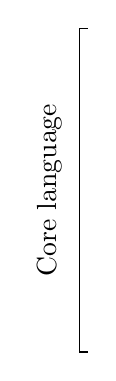
\begin{tikzpicture}\draw (0,0) -- ++(-1mm,0) -- ++(0,-11.7em) {} node[midway,anchor=base,xshift=-3mm,rotate=90] {Core language} -- ++(1mm,0);\end{tikzpicture}} &
  \typerule{e=v \qquad \Gamma,v:\T_1\vdash e:\T_0}
           {\Gamma,v:\T_1 ~\vdash~ e:\T_0\sqcap\T_1} &
  \typerule{e=e_1\,e_2 \qquad \Gamma \vdash e:\T, ~ e_1:\T_1, ~ e_2:\T_2\to\S_2}
           {\renewcommand\arraystretch{1.2}
            \begin{array}[t]{@{}l@{}l@{}}
              \Gamma ~\vdash~ & e:\T\sqcap\S_2, \\ 
                              & e_1:\T_1\sqcap\T_2, \\
                              & e_2:(\T_1\to\T)\sqcap(\T_2\to\S_2)
            \end{array}} & \\
  &
  \cspan2{
  \typerule{e=(v:\T)\mapsto e_1 \qquad \Gamma\vdash e:\T_0\to\S_0 \qquad \Gamma,v:\T\sqcap\T_0\vdash e_1:\T_1}
           {\renewcommand\arraystretch{1.2}
            \begin{array}[t]{r@{}l}
              \Gamma ~\vdash~ & e:(\T_0\to\S_0)\sqcap(\T\to\T_1)\\
              \Gamma,v:\T\sqcap\T_0 ~\vdash~ & e_1:\T_1\sqcap\S_0 
            \end{array}}  } & \\
  %
  \multirow{2}{1cm}[-1.8em]{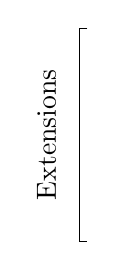
\begin{tikzpicture}\draw (0,0) -- ++(-1mm,0) -- ++(0,-7.7em) node[midway,anchor=base,xshift=-3mm,rotate=90] {Extensions} -- ++(1mm,0);\end{tikzpicture}} &
  \typerule{e=\fix e_1 \qquad \Gamma\vdash e:\T, ~ e_1:\T_1\to\T_2}          % fix
           {\Gamma\vdash e: \T\sqcap\T_2} &
  \typerule{e=e_1/e_2 \qquad \Gamma\vdash e:\T, ~ e_1:\T_1, ~ e_2:\T_2}      % /
           {\renewcommand\arraystretch{1.2}
            \begin{array}[t]{@{}l@{}l@{}}
              \Gamma\vdash{} & e_1:\T_1\sqcap\T, ~ e_2:\T_2\sqcap\T
            \end{array}} & \\
  &
  \typerule{e=[e_1]_{_{cond}} \qquad \Gamma\vdash e:\T,e_1:\T_1}                           % ::
           {\Gamma\vdash e:\T\sqcap\T_1, ~ e_1:\T\sqcap\T_1} &
  \typerule{e=e_1::\T \qquad \Gamma\vdash e:\T_0,e_1:\T_1}                           % ::
           {\Gamma\vdash e:\T\sqcap\T_0\sqcap\T_1, ~ e_1:\T\sqcap\T_0\sqcap\T_1}
\end{array}
\]
\caption{\label{lang:type refinement rules}
  Type refinement rules, for inferring qualifiers in sub-expressions.}
\end{figure*}

Note that two syntactically identical terms in different sub-trees may be assigned
different types by this method. This is a desirable property, as (some) context information
gets encoded in the type that way.

\examplePar Let $I_0\subseteq I$ be a unary predicate, and $0:T$ a constant.
The expression $f\,(i:I_0)\mapsto f\,i\,i ~/~ 0$ will induce the following type
inferences:

\hspace*{\fill}
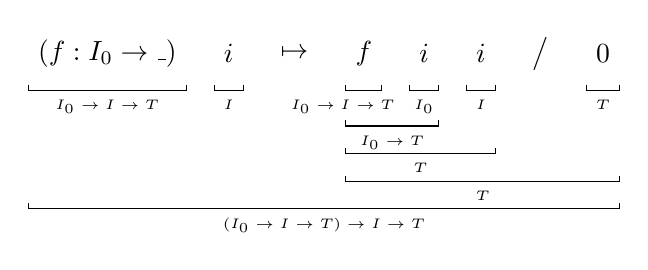
\begin{tikzpicture}[node distance=1em]
  \node(farg) {$(f:I_0\to\_)$};
  \node(iarg)[right=of farg] {$i$};
  \node(mapsto)[right=of iarg] {$\mapsto$};
  \node(f)[right=of mapsto] {$f$};
  \node(i1)[right=of f] {$i$};
  \node(i2)[right=of i1] {$i$};
  \node(slash)[right=of i2] {$\big/$};
  \node(zero)[right=of slash] {$0$};
  \node(l0)[coordinate,below=1mm of farg] {};
  \node(l1)[coordinate,below=4.5mm of l0] {};
  \node(l2)[coordinate,below=3.5mm of l1] {};
  \node(l3)[coordinate,below=3.5mm of l2] {};
  \node(l4)[coordinate,below=3.5mm of l3] {};
  \def\ytip{2pt}
  \draw (l0 -| farg.west) -- +(0,-\ytip) -| (l0 -| farg.east) node[pos=0.25,below] {\tiny $I_0\to I\to T$};
  \draw (l0 -| iarg.west) -- +(0,-\ytip) -| (l0 -| iarg.east) node[pos=0.25,below] {\tiny $I$};
  \draw (l0 -| f.west) -- +(0,-\ytip) -| (l0 -| f.east) node[pos=0.5,anchor=23,inner xsep=0] {\tiny $I_0\to I\to T$};
  \draw (l0 -| i1.west) -- +(0,-\ytip) -| (l0 -| i1.east) node[pos=0.25,below] {\tiny $I_0$};
  \draw (l0 -| i2.west) -- +(0,-\ytip) -| (l0 -| i2.east) node[pos=0.25,below] {\tiny $I$};
  \draw (l0 -| zero.west) -- +(0,-\ytip) -| (l0 -| zero.east) node[pos=0.25,below] {\tiny $T$};
  \draw (l1 -| f.west) -- +(0,-\ytip) -| (l1 -| i1.east) node[pos=0.25,below] {\tiny $I_0\to T$};
  \draw (l2 -| f.west) -- +(0,-\ytip) -| (l2 -| i2.east) node[pos=0.25,below] {\tiny $T$};
  \draw (l3 -| f.west) -- +(0,-\ytip) -| (l3 -| zero.east) node[pos=0.25,below] {\tiny $T$};
  \draw (l4 -| farg.west) -- +(0,-\ytip) -| (l4 -| zero.east) node[pos=0.25,below] {\tiny $(I_0\to I\to T)\to I\to T$};
\end{tikzpicture}
\hspace*{\fill}


\exampleTitle  \begin{comment}\subsection{Example}\end{comment}

\noindent
The specification of the Simplified Arbiter (\Cref{overview:arbiter spec}) will be written as
%
\[
  \renewcommand\arraystretch{1.5}
  \begin{array}{@{}l@{}l@{}l@{}}
    \lspan3{\xw{} : ((I\times I)\cap{<})\to J\to\R} \\
    \lspan3{\yw{} : ((J\times J)\cap{<})\to I\to\R} \\
    G ~=~ \fix \theta\,i\,j\mapsto{}
      & \lspan2{\big[0\big]_{i=j=0} \,\Big/~ \big[\yw{0j0}\big]_{i=0} \,\Big/~ \big[\xw{0i0}\big]_{j=0} \,\Big/} \\
      & \min~\langle~ & \min p\mapsto\theta_{pj}+\xw{pij}, \\
      & & \min q\mapsto\theta_{iq}+\yw{qji} ~\rangle
  \end{array}
\]

\medskip
We are using $f_{xy}$
as a more readable alternative typography for $f\,x\,y$,
where $f$ is a function symbol and $x$, $y$ are its arguments.

Note that the ranges for $\min p$ and $\min q$ are implicit, from the types of
$\xw{}$, $\yw{}$: \[\xw{pij}\neq\bot\implies p<i \quad \mbox{and} \quad \yw{qji}\neq\bot\implies q<j\]

\medskip
\hrule

\section{Tactics}
\label{tactics}

We now define the method by which that our framework transforms program terms, by means of \newterm{tactics}.
A tactic is a scheme of equalities that can be used for rewriting.
When applied to a program term, any occurrence of the {\bf left-hand side} is replaced by the {\bf right-hand side}.%
\footnote{This is also a standard convention in Coq, for example.}
A valid application of a tactic is an instance of the scheme that is well-typed and logically valid
(that is, the two sides have the same interpretation in any structure that interprets the free
variables occurring in the equality).

The application of tactics yields a sequence of program terms, each of which is checked to
be equivalent to the previous one. We refer to this sequence by the name \newterm{development}.

We associate with each tactic some \newterm{proof obligations}, listed after the word \textbf{\textit{Obligations}}
in the following paragraph.
When applying a tactic instance, these obligations are also instantiated and given to an automated prover. 
If verified successfully, they entail the validity of the instance. 
Clearly the tactic itself can be used as its proof obligation, if it is easy enough to prove automatically; 
in such cases we write ``\textbf{\textit{Obligations}:} tactic.''

The following are the major tactics provided by our framework. 
More tactic definitions are given in the appendix.

\newcommand\Obligations{\medskip\noindent\textbf{\textit{Obligations}:} }
\newcommand\reduce{\operatorname{reduce}}
\newcommand\listConcat{{\scriptstyle \,++\,}}

\theoremstyle{definition}
\newtheorem{tactic}{Tactic}

\newcommand\tacticdef[1]{\subsection*{\sf\larger #1}\vspace{-3mm}}
\newcommand\tacticdefcompact[1]{\medskip\noindent{\sf\larger #1}\medskip\hfill}

\tacticdefcompact{Slice} \label{tactics:Slice}
$f ~=~ \big[f\big]_{X_1} ~\Big/~ \big[f\big]_{X_2} ~\Big/ ~\cdots~ \Big/~ \big[f\big]_{X_r}$\hspace{10mm}

This tactic partitions a mapping into sub-regions. Each $X_i$ may be a cross product ($\times$)
according to the arity of $f$.

\Obligations tactic.

Informally, the recombination expression is equal to $f$
when $X_{1..r}$ ``cover'' all the defined points of $f$ (also known as the \newterm{support} of $f$).

\medskip
\tacticdefcompact{Stratify}
$\fix (f\applt g) ~=~ (\fix f) ~\applt~ \big(\psi\mapsto \fix (\widehat\psi\applt g)\big)$
\\
where $\widehat\psi$ abbreviates $\theta\mapsto\psi$, with fresh variable $\theta$.

This tactic is used to break a long (recursive) computation into simpler sub-computations.
$\psi$ may be fresh, or it may reuse a variable already occurring in $g$, rebinding those occurrences.
An example is required to understand why this is useful.

Let $h=\theta\mapsto\big([t_0]_{I_0}\big/[t_1]_{I_1}\big)$, where $t_{0,1}$ are terms with free variable $\theta$.
Stratification is done by setting $f=\theta\mapsto t_0$ and
 $g=f\,\theta\mapsto [f\,\theta]_{I_0}\big/[t_1]_{I_1}$. We get $\fix h=\fix(f\applt g)$; {\sf~Stratify}
breaks it into $\fix f$ and $\psi\mapsto \fix (\widehat\psi\applt g)$,
which get simplified with $\beta$-reduction, giving the expression the form:

\vspace{-5mm}
\[\big(\fix(\theta\mapsto t_0)\big) ~\applt~ 
  \Big(\psi\mapsto \fix \big(\theta\mapsto[\psi]_{I_0}\big/[t_1]_{I_1}\big)\Big)\]

\vspace{-2mm}
This precisely encodes our intuition of computing the fixed point of $t_0$ first,
then $t_1$ based on the result of $t_0$.

\Obligations Let $h=f\applt g$ and $g'=\psi\mapsto\widehat\psi\applt g$. Let $\theta,\zeta$ be
fresh variables.
\begin{equation}
\renewcommand\arraystretch{1.5}
\begin{array}{l@{\qquad}l}
f\,(g'\,\zeta\,\theta) ~=~ f\,\zeta &
g'\,(f\,\theta)\,\theta ~=~ h\,\theta
\end{array}
\label{tactics:Stratify obligations}
\end{equation}

Proof is given in \Cref{tactics:soundness}.

\tacticdef{Synth} \label{tactics:Synth}
\[\fix\big(h_1 ~\big/~ \cdots ~\big/~ h_r\big) ~=~ 
  f_1 :: \T_1 ~\big/~ \cdots ~\big/~ f_r :: \T_r\]

This tactic is used to generate recursive calls to sub-programs. For $i=1..r$, $f_i$
is one of the following: $\fix h_i$, $h_i\,\psi$, or $t\,\psi$, where $\psi$ is some
variable and $t$ is a term corresponding to a previously defined subroutine
($A$, $B$, $C$ in the example).
Bellmania chooses these values automatically (see \Cref{tactics:synthesis}),
but the user may override it.

\newcommand\Y{\mathcal{Y}}

\Obligations Let $h=h_1/\cdots/h_r$, and let $\T\to\T$ be the shape of $h$. 
  For each $f_i$, depending on the form of $f_i$:
\begin{itemize}
  \item If $f_i \cong \fix f$ --- \\
    \rule{0pt}{12pt}
    $h :: (\T \to \Y) = h :: (\Y \to \Y) = g :: (\Y \to \T)$
    for some $\Y$ which is a subtype of $\T$ and a supertype of $\T_i$.
  \item If $f_i$ does not contain any ``$\fix$'' terms ---\\
    \rule{0pt}{12pt}
    $h\,(h\,\theta) :: \T_i = f_i :: \T_i$ for a fresh variable $\theta$.
\end{itemize}

We use $\cong$ to denote syntactic congruence up to $\beta$-reduction.

\begin{comment}
\Obligations Let $h=h_1/\cdots/h_r$, let $\overline\theta\!=\!\theta_{1..r}$ be $r$ fresh variables, and let
$f = \theta_{1..r} \mapsto (f_1\,\theta_1)::\T_1/\cdots/(f_r\,\theta_r)::\T_r$.
\begin{itemize}
  \item $\T_{1..r}$ are disjoint mappings.
  \item {\bf Either}\quad $h\,(f\,\overline\theta) = f\,\overline\theta$ \\{\bf or}\qquad
  $\begin{array}[t]{l} h\,\theta=\theta ~\limplies~ (f_i\,\theta :: \T_i)=\theta :: \T_i ~, \\
  \theta::\T_1~/~\cdots~/~\theta::\T_r=\theta\end{array}$
\end{itemize}

(We give two alternatives, as the first is usually easier to prove, but may hold in less cases)
\end{comment}


\newenvironment{tacticbox}[1]{\begin{center}
  \begin{tabular}{|@{~~~~}l@{~~~~}|}\hline
    \rule{0pt}{2.3ex}\underline{\sf \,#1\,}\\[.4em]$}
  {$\\[-1em] \\[.3ex] \hline \end{tabular} \end{center}}


\subsection{Synthesis-supported {\sf Synth} Tactic}
\label{tactics:synthesis}

As mentioned in \Cref{intro,overview}, the user is assisted by automatic
inference while applying tactics. In particular, the {\sf Synth} tactic requires
the user to specify a subroutine to call and parameters to call it with.
In addition, the subtype $\Y$ is required to complete the correctness proof.
To automate this task, Bellmania employs {\cegis}, a software synthesis technique
implemented in the tool {\Sketch}~\cite{STTT13/Solar-Lezama}. The proof obligations, along with the possible
space of parameter assignments taken from the set of sub-types defined during
{\sf Slice}, are translated to {\Sketch}. Since {\Sketch} uses bounded domains,
the result is then verified using full SMT.

While the size of the search space is not huge, typically in the order of \textasciitilde50
alternatives, it is usually hard for the user to figure out which exact call
should be made. Since {\sf Synth} is used extensively throughout the develoment,
This kind of automation greatly improves overall usability.

\subsection{Soundness}
\label{tactics:soundness}

\renewenvironment{proof}{\noindent{\bf Proof.~}}{}

\begin{theorem}
Let $s=s'$ be an instance of one of the tactics introduced in this section.
let $a_i=b_i$, $i=1..k$, be the proof obligations. If $\semp{a_i}=\semp{b_i}$
for all interpretations of the free variables of $a_i$ and $b_i$, then
$\semp{s}=\semp{s'}$ for all interpretations of the free variables of $s$ and $s'$.
\end{theorem}

\begin{proof}
For the tactics with \textbf{\textit{Obligations}:} tactic, the theorem is trivial.

\medskip
\noindent
{\tt >} For {\sf Stratify}, let $f$, $g$ be partial functions such that
\vspace{-.5em}
\[\renewcommand\arraystretch{1.3}
  \forall \theta,\zeta.\quad \begin{array}{l}f\,(g\,\zeta\,\theta) ~=~ f\,\zeta \quad\land\quad
  g\,(f\,\theta)\,\theta ~=~ h\,\theta
  \end{array}\quad\]
  
Assume that $\zeta = \fix f$ and $\theta = \fix (g\,\zeta)$. 
That is, $f\,\zeta = \zeta$ and $g\,\zeta\,\theta = \theta$.
Then ---
\vspace{-.5em}
\[\renewcommand\arraystretch{1.3}
  \begin{array}{l@{}l}
   h\,\theta & {}= g\,(f\,\theta)\,\theta = g\,(f\,(g\,\zeta\,\theta))\,\theta =
              g\,(f\,\zeta)\,\theta = \theta
  \end{array}\]
  
\noindent
So $\theta = \fix h$. We get $\fix h = \fix \big(g \,(\fix f)\big)$; equivalently,
\[\fix h = (\fix f) \applt \big(\psi\mapsto\fix (g\,\psi)\big)\]

Now instantiate $h$, $f$, and $g$, with $f\applt g$, $f$, and $g'$ from \Cref{tactics:Stratify obligations},
and we obtain the equality in the tactic.

\medskip
\noindent
{\tt >} For {\sf Synth}, ({\it i}) assume $f_i=\fix g$ and
\[h :: \T\to\Y = h :: \Y\to\Y = g :: \Y\to\T\]

Intuitively, $\Y$ ``cuts out'' a region of an array $\theta :: \T$ given
as input to $h$ and $g$. This area is self-contained, in the sense that
only elements in $\Y$ are needed to compute elements in $\Y$, as indicated
by the refined type $\Y\to\Y$.

Notice that from the premise follows $g :: \Y\to\T = g :: \Y\to\Y$. We use the following corollary:

\medskip\noindent
{\bf Corollary.~} Let $f : \T\to\T$; if either $f :: \T\to\Y = f :: \Y\to\Y$ or $f :: \Y\to\T = f :: \Y\to\Y$, 
then $(\fix f)::\Y = \fix (f :: \Y\to\Y)$.

Proof is included in the appendix.

\medskip
From the corollary, and for the given $h$ and $g$, we learn that $(\fix h)::\Y = \fix(h::\Y\to\Y)$,
and also $(\fix g)::\Y=\fix(g::\Y\to\Y)$. Since $h::\Y\to\Y=g::\Y\to\Y$,
we get $(\fix h)::\Y = (\fix g)::\Y$; now, $\Y$ is a supertype of $\T_i$, so $(\theta::\Y)::\T_i=\theta::\T_i$:
\[\renewcommand\arraystretch{1.3}
  \begin{array}{l}(\fix h)::\T_i = ((\fix h)::\Y)::\T_i = ((\fix g)::\Y)::\T_i = \\
    \qquad = (\fix g)::\T_i=f_i::\T_i
  \end{array}\]

{\it (ii)} Assume $h\,(h\,\theta) :: \T_i = f_i :: \T_i$ holds for any $\theta:\T$,
then in particlar, for $\theta=\fix\,h$, we get $h\,(h\,\fix h) :: \T_i = f_i :: \T_i$.
Since $h\,(h\,\fix h) = \fix h$, we obtain the conjecture $(\fix h) :: \T_i = f_i :: \T_i$.
\qed
\end{proof}

\medskip
Our reliance on the termination of $\fix$ expressions may seem conspicuous, since some of these
expressions are generated automatically by the system. However, a closer look reveals that whenever
such a computation is introduced, the set of the recursive calls it makes is a subset of those made by the existing one.
Therefore, if the original recurrence terminates, so does the new one. In any case, all the recurrences
in our development have a trivial termination argument (the indexes $i$,$j$ change monotonically between calls),
so practically, this should never become a problem.

\newcommand\vtyped[2]{\underset{\scriptscriptstyle ( #2 )}{ #1 }}


\input{05-automated}
\section{Code Generation}
\label{codegen}

We built a compiler for programs in Bellmania language that generates efficient C++ code parallelized with Intel Cilk constructs. The compiler uses type information from the development to improve the
quality of generated code. From the types of sub-terms corresponding
to array indices, the compiler extracts information about what region
of the array is read by each computation, and from the types of $\lambda$-bound index variable it constructs loops that write to
the appropriate regions. The compiler utilizes the SMT solver to infer dependency constraints as in~\cite{JACM67/Karp},
and figures out the direction of each loop (ascending or descending). 
In addition, inter-quadrant dependencies can be used to determine which computations can be run in parallel (at the granularity of
function calls) based on a fork-join model;
two calls are considered non-conflicting if each write region is disjoint from the others' read and write regions.
Disjointness can be decided using propositional logic through the predicate abstraction induced by type qualifiers.

The compiler also employs more traditional optimization techniques
to further simplify the code and improve its running time:
(1) lifts conditionals to loop bounds via simple interval analysis, %to optimize the loop bounds and performs some traditional compiler %transformations to reduce the number of iterations and comparisons,
(2) eliminates redundant iterations and comparisons that can be resolved at compile time,
and (3) identifies loops that read non-contiguous memory blocks and applies copy optimization~\cite{ASPLOS91/Lam} automatically to better utilize caches. Examples of generated code are included in the supplemental material with this submission.

 
%Use Cilk for parallelization - references later
%Using SMT solver and type information to find directions of loops for fixed point computations
%Using type information and SMT solvers to parallelize different components
%Using type information to optimize the loop bounds, reduce checking of guards and do copy optimization
%Traditional compiler transformations

%code can be found in repo
%JACM67: Recurrences to loops: http://dl.acm.org/citation.cfm?id=321418
%ASPLOS1991: copy optimization: http://suif.stanford.edu/papers/lam-asplos91.pdf
\section{Empirical Evaluation}

We implemented our technique and used it to generate cache-oblivious
divide-and-conquer implementations of three algorithms that were used as
benchmarks in \cite{IPDPS15/Tithi}, and a few others.

\begin{paragraph}{Gap problem.}
A generalized minimal edit distance problem. Given two input strings 
$\overline{x}=x_1\cdots x_m$ and $\overline{y}=y_1\cdots y_n$,
compute the cost of transforming $x$ into $y$ by any combination of the
following steps
\begin{itemize}
  \item Replacing $x_i$ with $y_j$, at cost $c_{ij}$.
  \item Deleting $x_{p+1}\cdots x_q$, at cost $\xw{pq}$.
  \item Inserting $y_{p+1}\cdots y_q$ in $\overline{x}$, at cost $\yw{pq}$.
\end{itemize}
\end{paragraph}

\begin{paragraph}{Parenthesis problem.} Compute
an optimal placements of parenthesis in a long chain of multiplication, e.g. of matrices, where the input is
are cost functions $x_i$ for accessing the $i$-th element and
$w_{ikj}$ for multiplying elements $[i,k)$ by elements $[k,j)$.
The corresponding recurrence is shown in \Cref{evaluation:paren spec}.
\end{paragraph}

\begin{paragraph}{Protein Accordion Folding problem.} A protein can be viewed
as a string $\mathcal{P}_{1..n}$ over an alphabet of amino acids. 
The protein folds itself in a way that minimizes potential energy.
Some of the acids are {\em hydrophobic}; minimization of the total hydrophobic
area exposed to water is a major driving force of the folding process.
One possible model is packing $\mathcal{P}$ in a two-dimensional square lattice
in a way that maximizes the number of pairs of hydrophobic elements,
where the shape of the fold is an {\em accordion}, alternating between going down and going
up.
\end{paragraph}

\medskip
We also exercised our system on a number of textbook problems:
the Longest Common Subsequence (LCS) problem, the Knapsack problem,
and the Bitonic Traveling Salesman problem.

\begin{figure}
\[
  \renewcommand\arraystretch{1.5}
  \begin{array}{@{}l@{}l}
    \lspan2{x :: J\to\R} \\
    \lspan2{w :: (J\times J\times J)\to\R} \\
    E ~=~ \fix \theta\,i\,j\mapsto{}
      & {\big[x_{ij}\big]_{i+1=j} ~\Big/~} \\
      & \min k\mapsto\theta_{ik}+\theta_{kj}+w_{ikj} \\
  \end{array}
\]
\caption{\label{evaluation:paren spec}
  Specifications for the Parenthesis Assignment DP problem.}
\end{figure}


The tactic application engine is implemented in Scala. We implemeted a prototype
IDE using HTML5 and AngularJS, which communicates with the engine by sending
and receiving program terms serialized as JSON. Our system supports using either
Z3 or CVC4 as the back-end SMT solver for discharging proof obligations required
for soundness proofs. Synthesis of recursive calls is done by translating the
program to Sketch, which employs CEGIS to find the correct assignment to parameters.
To argue for the feasibility of our system, we include
solver running time for the verification of the three most used tactics,
as well as time required for Sketch synthesis, in \Cref{evaluation:solving time}.
We consider an average delay of \textasciitilde 10 seconds to be reasonable, even for an interactive
environment such as Bellmania. 

The compiler for programs in Bellmania is implemented in 
python and generates C++ code with Intel Cilk constructs for parallelization.
Table~\ref{evaluation:cppruntimes} shows performance improvement for our 
auto-generated implementation (AUTO) on the state-of-the-art optimized parallel
loop implementation (LOOPDP) from~\cite{IPDPS15/Tithi}. It also compares AUTO with manually 
optimized recursive implementations CO\_Opt and COZ from~\cite{IPDPS15/Tithi}. 
Bellmania compiler automatically does \textit{copy optimization} 
as done in CO\_Opt and COZ. COZ also incorporates some low-level 
optimizations like using a Z-order layout of the array etc.,
which are out of scope for this paper. %pointer arithmetics for loop traversal? 
%Explicit vectorization of loops?
$N$ is the problem size and $B$ is the base case size for using loops 
instead of recursion. It can be seen from the table that our implementation 
performs close to the manually optimized code and can be optimized further by 
hand. Figure~\ref{fig:gap} depicts the performance of these implementations 
on one sample instance
as a function of problem size and shows the scalability of our technique. %ROHIT:scalability of what:the technique or the code?

\begin{table}
\centering
\begin{tabular}{|l|c|c|c|}
    \cline{2-4}
  \multicolumn{1}{c|}{} & \multicolumn{3}{c|}{\scriptsize Speedup w.r.t parallel LOOPDP on 6 cores}  \\
  \multicolumn{1}{c|}{} & \multicolumn{3}{c|}{\scriptsize   CPU (12 workers), N=16384, B=64}  \\
  \multicolumn{1}{c|}{} & \multicolumn{1}{c|}{~~~\sf CO\_Opt~~~} & \multicolumn{1}{c|}{~~~~\sf COZ~~~~} & \multicolumn{1}{c|}{\sf AUTO}  \\
  \hline
  {\bf Gap}  & 21x & 34x & 30x\\
  \hline
  {\bf Parenthesis}  & 32x & 50x & 46x\\
  \hline
  {\bf Protein} & 2.2x & 2.6x & 1.4x \\
  \hline
  %{\bf LCS} & 10x &  10x  &  10x \\
  %\hline
  {\bf Knapsack} & $-$ & $-$ & ?x\\
  \hline
  %{\bf Bitonic} & & 2 & \\
  %\hline
\end{tabular}
\caption{\label{evaluation:cppruntimes}
  Performance of different C++ implementations}
\end{table}


\begin{table}
\centering
\renewcommand\a{({\it i})}    % relax! it's only for this figure
\renewcommand\b{({\it ii})}
\renewcommand\c{({\it iii})}
\begin{tabular}{|l|r|rrr|r@{\quad}|}
  \cline{2-6}
  \multicolumn{1}{c|}{} &    & \multicolumn{4}{c|}{\small Average solving time ({\it s})}  \\
  \multicolumn{1}{c|}{} &    & \multicolumn{3}{c|}{\small Verification} & \multicolumn{1}{@{\,}c@{\,}|}{\small Synthesis} \\
  \multicolumn{1}{c|}{} & \# & \multicolumn{1}{c|}{~\sf Slice~} & \multicolumn{1}{c|}{\sf Stratify} & \multicolumn{1}{c|}{\sf Synth} & \multicolumn{1}{c|}{Sketch} \\
  \hline
  {\bf Gap                 }  &  3  &  1.5  &  6.4   &   0.2  &  8     \\
  \hline
  {\bf Paren               }  &  3  &  0.8  &  16.5   &   0.8  &  11.2     \\
  \hline
  {\bf Accordion           }  &  4  &  0.6  &  3.8   &   0.4  &  6.1     \\
  \hline
  {\bf LCS                 }  &  1  &  0.2  &  1.5   &   0.4  &  3.1     \\
  \hline
  {\bf Knapsack            }  &  2  &  0.3  &  1.6   &   0.4  &  4.6     \\
  \hline
  {\bf Bitonic             }  &  3  &  0.7  &  1.9   &   0.7  &  6.4     \\
  \hline
\end{tabular}
\caption{\label{evaluation:solving time}
  Average proof search time for proof obligations and synthesis
  time}
\end{table}



\begin{figure}
\begin{tikzpicture}
	\begin{axis}[
	    title=Parenthesis,
	    ymode=log,
		xlabel=$n$,
		ylabel=Time ({\it s}),
		scaled x ticks=false, %{real:1000}
		log basis y=2, ymajorgrids=true]
	\addplot[color=blue!50!white,ultra thick,mark=*,smooth] table[x=n/Time(s),y=COZ] {data/plot1.dat}
	  [yshift=-8pt] node[pos=0] {CO};
	\addplot[color=red!70!white,ultra thick,mark=*,smooth] table[x=n/Time(s),y=Tiled/Par] {data/plot1.dat}
	  [yshift=-10pt] node[pos=0] {PluTo};
	\end{axis}
\end{tikzpicture}
\begin{tikzpicture}
	\begin{axis}[
	    title=Gap,
	    ymode=log,
		xlabel=$n$,
		scaled x ticks=false, %{real:1000}
		log basis y=2, ymajorgrids=true]
	\addplot[color=blue!50!white,ultra thick,mark=*,smooth] table[x=n/Time(s),y=COZ] {data/plot2.dat}
	  [yshift=-8pt] node[pos=0] {CO};
	\addplot[color=red!70!white,ultra thick,mark=*,smooth] table[x=n/Time(s),y=Tiled/Par] {data/plot2.dat}
	  [yshift=-8pt] node[pos=0] {PoCC};
	\end{axis}
\end{tikzpicture}
\begin{tikzpicture}
	\begin{axis}[
	    title=Floyd-Warshall,
	    ymode=log,
		xlabel=$n$,
		scaled x ticks=false, %{real:1000}
		log basis y=2, ymajorgrids=true]
	\addplot[color=blue!50!white,ultra thick,mark=*,smooth] table[x=n/Time(s),y=COZ] {data/plot3.dat}
	  [yshift=-8pt] node[pos=0] {CO};
	\addplot[color=red!70!white,ultra thick,mark=*,smooth] table[x=n/Time(s),y=Tiled/Par] {data/plot3.dat}
	  [yshift=-8pt] node[pos=0] {PoCC};
	\end{axis}
\end{tikzpicture}

\caption{\label{fig:gap} Performance comparison for parallelized implementations for Gap problem on 6-core Intel i7 CPU}
\end{figure}
\section{Related Work}
\label{related}

Classical work by Smith \etal~\cite{AI85/Smith} presents rule-based transformation, stringing it
tightly with program verification. This lay the foundation for semi-automatic programming~\cite{CPS91/Blaine,TSE90/Smith,TPHOLs96/Butler}.
More recently, a similar approach was introduced into Leon~\cite{OOPSLA13/Kneuss}, leveraging deductive
tools as a way to boost {\cegis}, thereby covering more programs. Bellmania takes a dual approach, where
automated techniques based on SMT are leveraged to support and improve deductive synthesis.

Inductive synthesis has been the focus of renewed interest thanks to the discovery of techniques that leverage SAT/SMT solvers to symbolically represent and search very large spaces of possible programs~\cite{APLAS09/Solar-Lezama, PLDI11/Gulwani, Onward13/Torlak},
and the use of counterexample-guided inductive synthesis ({\cegis}), which allows one to leverage inductive techniques to find programs that satisfy more general specifications. 
Our work is also inspired by the StreamBit project~\cite{PLDI05/Solar-Lezama}, which
introduced the idea of transformation rules with missing details that can be inferred by a symbolic search procedure.

Fiat~\cite{POPL15/Delaware} is another recent system that admits stepwise transformation of specifications
into programs via a refinement calculus. While Bellmania offloads proofs to SMT and \Sketch{},
Fiat uses decision procedures in Coq,
reling heavily on deductive reasoning and uses Ltac scripts for automation.
The intended users of Fiat is regular software developers who invoke pre-packaged scripts,
whereas Bellmania targets domain experts who exercise more control over the generated code.

Broadly speaking, the Bellmania system could have been implemented as a library on top of a framework
such as Coq or Why3~\cite{ESOP13/Filliatre} using binding to SMT solvers provided by these frameworks.
The decision not to do so was merely a design choice, to facilitate easier integration with our UI and with \Sketch{}.

Polyhedral compilers offer some optimizations for the same domain of problem via tiling~\cite{HPC10/Pouchet,PLDI08/Bondhugula}.
While showing significant speedups, these compilers cannot produce divide-and-conquer optimizations,
which were proved to be more effective by \cite{IPDPS15/Tithi}.

Autogen~\cite{PPoPP16/Chowdhury} is a most recent advance that employs dynamic analysis to discover
a program's access pattern and learn a decomposition that can be used to generate a divide-and-conquer
implementation. The two methods are complementary, since Autogen does not provide correctness guarantees, so the user might be able to use insights from Autogen while developing certified code in Bellmania.

Pu \etal{}~\cite{OOPSLA11/Pu} have shown that recurrences for DP can be generated automatically from a non-recursive specification of the optimization problem.
This is orthogonal; in Bellmania, the recurrence is the input, and the output is an efficient divide-and-conquer implementation.

\begin{comment}
Our ``$\big/$'' operator can be compared to the separating disjunction ``$\ast$'' of Separation Logic~\cite{LICS02/Reynolds},
used to frame parts of the dynamic heap (which can be thought of as one large array),
in particular while checking that a program only accesses the parts allocated to it in its precondition.
While $\ast$ has the semantics of an existentially quantified predicate, Bellmania uses type qualifiers
to explicitly specify a formula defining each part. In this sense, it is more closely related to
Region Logic~\cite{ECOOP08/Banerjee}. These formulas make encoding in first-order logic straightforward,
and the use of Liquid Types allows for any number of dimensions and for decidable checking of domain inclusion
and disjointness.
\end{comment}
\section{Conclusion}
\label{conc}

The examples in this paper show that a few well-placed tactics can cover a wide range
of program transformations. The introduction of solver-aided tactics allowed us to make
the library of tactics smaller, by enabling the design of higher-level, more generic
tactics. Their small number gives the hope that end-users with some mathematical background
will be able to use the system without the steep learning curve that is usually associated
with proof assistants. This can be a valuable tool for algorithms research.

\begin{comment}
Moreover, limiting the number of tactics shrinks the space in which to search for programs,
so that an additional level automation may be achieved via AI or ML methods. As more
developments are done by humans and collected in a database, those algorithms would become
more adept in predicting the next step of the construction.
\end{comment}

But solver-aided tactics should not be seen as specific to divide-and-conquer algorithms,
or even to algorithms. The same approach can be applied to other domains. Domain knowledge
can be used to craft specialized tactics, providing users with the power to use a high-level
DSL to specify their requirements, without sacrificing performance.


\bibliographystyle{abbrvnat}
\bibliography{oopsla2016}
% The bibliography should be embedded for final submission.

%\begin{thebibliography}{}
%\softraggedright

%\bibitem[Smith et~al.(2009)Smith, Jones]{smith02}
%P. Q. Smith, and X. Y. Jones. ...reference text...

%\end{thebibliography}


\end{document}
